\documentclass[11pt]{article}
\usepackage[a4paper,margin=23mm]{geometry}
\usepackage{fontspec}
\setmainfont{TeX Gyre Pagella}
\setsansfont{TeX Gyre Heros}
\setmonofont{Inconsolata}
\usepackage{amsmath,amssymb,booktabs,longtable,tabularx,enumitem}
\usepackage{tikz,float}
\usetikzlibrary{arrows.meta,positioning,fit,calc}
\usepackage{xcolor,hyperref,xurl}
\hypersetup{colorlinks=true,linkcolor=blue!45!black,urlcolor=blue!45!black,
  pdftitle={Kayfabe v3: an architecture to argue with},pdfauthor={Kayfabe project}}
\setlength{\emergencystretch}{3em}
\setlength{\parskip}{0.45em}
\setlength{\parindent}{0pt}
\setlist{nosep,leftmargin=*}
\newcommand{\baseline}{12c4008705f17033a803e56d4d479bf1275cdb94}
\newcommand{\repobase}{https://github.com/reindertpelsma/kayfabe}
\newcommand{\code}[1]{\texttt{\detokenize{#1}}}
\newcommand{\sourceentry}[3]{%
  \expandafter\def\csname source-number:#1\endcsname{#2}%
  \expandafter\def\csname source-url:#1\endcsname{#3}}
\newcommand{\reposource}[4]{\sourceentry{#1}{#2}{\repobase/blob/#3/#4}}
\newcommand{\src}[1]{\,\textsuperscript{\href{\csname source-url:#1\endcsname}
  {[\csname source-number:#1\endcsname]}}}
\newcommand{\readcode}{\textbf{CODE.} }
\newcommand{\doc}{\textbf{DOC.} }
\newcommand{\measured}{\textbf{MEASURED.} }
\newcommand{\reported}{\textbf{REPORTED.} }
\newcommand{\unmeasured}{\textbf{UNMEASURED.} }
\newcommand{\inferred}{\textbf{INFERRED.} }
\newcommand{\unverified}{\textbf{UNVERIFIED.} }
\newcommand{\evidence}[4]{\item\label{e:#1}\textbf{#1}: #4\\
  Revision \code{#2}.\\\href{\repobase/blob/#2/#3}{\nolinkurl{#3}}}
\newcommand{\attack}[3]{\textbf{Invariant:} #1\par
  \textbf{Tests and scope:} #2\par\textbf{What the test could miss:} #3\par}
\newcounter{question}
\newcommand{\question}[4]{\refstepcounter{question}
  \subsection*{Q\thequestion. #1}\textbf{Setup:} #2\par
  \textbf{Observation to obtain:} #3\par\textbf{Decision it changes:} #4\par}
\tikzset{concept/.style={draw,rounded corners,align=center,font=\small,
  text width=35mm,minimum height=12mm,fill=blue!4},
  flow/.style={-{Latex[length=2mm]},thick}}

% Generated from sources_v3.json; numeric citations link directly to pinned blobs.
\reposource{architecture}{1}{%
12c4008705f17033a803e56d4d479bf1275cdb94}{%
ARCHITECTURE.md}
\reposource{rules}{2}{%
12c4008705f17033a803e56d4d479bf1275cdb94}{%
AGENTS.md}
\reposource{debt}{3}{%
12c4008705f17033a803e56d4d479bf1275cdb94}{%
scripts/claim_ledger.py}
\reposource{readme}{4}{%
12c4008705f17033a803e56d4d479bf1275cdb94}{%
README.md}
\reposource{faq}{5}{%
12c4008705f17033a803e56d4d479bf1275cdb94}{%
docs/FAQ.md}
\reposource{credits}{6}{%
12c4008705f17033a803e56d4d479bf1275cdb94}{%
docs/howto/credits.md}
\reposource{notices}{7}{%
12c4008705f17033a803e56d4d479bf1275cdb94}{%
docs/NOTICES.md}
\reposource{license}{8}{%
12c4008705f17033a803e56d4d479bf1275cdb94}{%
LICENSE}
\reposource{security}{9}{%
12c4008705f17033a803e56d4d479bf1275cdb94}{%
docs/howto/security.md}
\reposource{windows}{10}{%
12c4008705f17033a803e56d4d479bf1275cdb94}{%
docs/WINDOWS_GUEST_SETUP.md}
\reposource{requirements}{11}{%
12c4008705f17033a803e56d4d479bf1275cdb94}{%
docs/howto/requirements.md}
\reposource{design}{12}{%
12c4008705f17033a803e56d4d479bf1275cdb94}{%
docs/design/THE_ARCHITECTURE_v3.md}
\reposource{rulings}{13}{%
12c4008705f17033a803e56d4d479bf1275cdb94}{%
docs/OWNER_RULINGS.md}
\reposource{handoff}{14}{%
12c4008705f17033a803e56d4d479bf1275cdb94}{%
docs/STATUS_AND_HANDOFF.md}
\reposource{status}{15}{%
12c4008705f17033a803e56d4d479bf1275cdb94}{%
docs/STATUS_DETAIL.md}
\reposource{old}{16}{%
12c4008705f17033a803e56d4d479bf1275cdb94}{%
docs/whitepaper/kayfabe_architecture.tex}
\reposource{translated}{17}{%
12c4008705f17033a803e56d4d479bf1275cdb94}{%
docs/design/THE_TRANSLATED_PLANE.md}
\reposource{kinds}{18}{%
12c4008705f17033a803e56d4d479bf1275cdb94}{%
docs/design/the_three_channel_kinds.md}
\reposource{gspcode}{19}{%
12c4008705f17033a803e56d4d479bf1275cdb94}{%
crates/kf-gsp/src/lib.rs}
\reposource{rmcode}{20}{%
12c4008705f17033a803e56d4d479bf1275cdb94}{%
crates/kf-rm/src/lib.rs}
\reposource{corecode}{21}{%
12c4008705f17033a803e56d4d479bf1275cdb94}{%
crates/kf-core/src/lib.rs}
\reposource{trapcode}{22}{%
12c4008705f17033a803e56d4d479bf1275cdb94}{%
crates/kf-trap/src/lib.rs}
\reposource{hostcode}{23}{%
12c4008705f17033a803e56d4d479bf1275cdb94}{%
crates/kf-host/src/lib.rs}
\reposource{memcode}{24}{%
12c4008705f17033a803e56d4d479bf1275cdb94}{%
crates/kf-mem/src/vasmgr.rs}
\reposource{diffcode}{25}{%
12c4008705f17033a803e56d4d479bf1275cdb94}{%
crates/kf-cuda/src/diffmodel.rs}
\reposource{applycode}{26}{%
12c4008705f17033a803e56d4d479bf1275cdb94}{%
crates/kf-mem/src/apply.rs}
\reposource{tsgcode}{27}{%
12c4008705f17033a803e56d4d479bf1275cdb94}{%
crates/kf-host/src/channel.rs}
\reposource{latejoin}{28}{%
12c4008705f17033a803e56d4d479bf1275cdb94}{%
docs/design/V3_LATE_TSG_JOINER.md}
\reposource{relaydesign}{29}{%
12c4008705f17033a803e56d4d479bf1275cdb94}{%
docs/design/V3_WINDOWS_USER_RING_RELAY.md}
\reposource{lifecycle}{30}{%
12c4008705f17033a803e56d4d479bf1275cdb94}{%
docs/design/V3_USER_RING_LIFECYCLE_20261016.md}
\reposource{eventloop}{31}{%
12c4008705f17033a803e56d4d479bf1275cdb94}{%
docs/design/V3_USER_RING_EVENT_LOOP_20261014.md}
\reposource{lazycode}{32}{%
12c4008705f17033a803e56d4d479bf1275cdb94}{%
crates/kf-chan/src/user_lazy.rs}
\reposource{turncode}{33}{%
12c4008705f17033a803e56d4d479bf1275cdb94}{%
crates/kf-chan/src/user_turn.rs}
\reposource{display}{34}{%
12c4008705f17033a803e56d4d479bf1275cdb94}{%
docs/design/V3_DISPLAY.md}
\reposource{planes}{35}{%
12c4008705f17033a803e56d4d479bf1275cdb94}{%
docs/design/V3_DISPLAY_PLANES_ORACLE.md}
\reposource{pacing}{36}{%
12c4008705f17033a803e56d4d479bf1275cdb94}{%
docs/design/V3_DISPLAY_PACING_20261017.md}
\reposource{video}{37}{%
12c4008705f17033a803e56d4d479bf1275cdb94}{%
docs/design/V3_VIDEO_ENGINES.md}
\reposource{uvmdesign}{38}{%
12c4008705f17033a803e56d4d479bf1275cdb94}{%
docs/design/V3_UVM_DEMAND_PAGING.md}
\reposource{driverdesign}{39}{%
12c4008705f17033a803e56d4d479bf1275cdb94}{%
docs/design/V3_DRIVER_MATRIX.md}
\reposource{constants}{40}{%
12c4008705f17033a803e56d4d479bf1275cdb94}{%
docs/design/V3_CONSTANT_STRATEGY.md}
\reposource{provenance}{41}{%
12c4008705f17033a803e56d4d479bf1275cdb94}{%
docs/design/V3_PROVENANCE.md}
\reposource{flags}{42}{%
12c4008705f17033a803e56d4d479bf1275cdb94}{%
docs/design/V3_FLAG_INVENTORY.md}
\reposource{cooperation}{43}{%
12c4008705f17033a803e56d4d479bf1275cdb94}{%
docs/design/V3_COOPERATIVE_TIERS.md}
\reposource{gaps}{44}{%
12c4008705f17033a803e56d4d479bf1275cdb94}{%
docs/design/V3_FEATURE_GAPS.md}
\reposource{reset}{45}{%
12c4008705f17033a803e56d4d479bf1275cdb94}{%
docs/design/V3_DEVICE_RESET.md}
\reposource{sleep}{46}{%
12c4008705f17033a803e56d4d479bf1275cdb94}{%
docs/design/V3_S3_RESUME.md}
\reposource{migrationdecision}{47}{%
12c4008705f17033a803e56d4d479bf1275cdb94}{%
docs/design/V3_WINDOWS_USER_FIFO_MIGRATION_DECISION_20261011.md}
\reposource{owed}{48}{%
12c4008705f17033a803e56d4d479bf1275cdb94}{%
docs/design/V3_ENS8_OWED_RING_TESTS.md}
\reposource{broker}{49}{%
12c4008705f17033a803e56d4d479bf1275cdb94}{%
ci/vast-broker/README.md}
\reposource{threat}{50}{%
12c4008705f17033a803e56d4d479bf1275cdb94}{%
ci/vast-broker/docs/THREAT_MODEL.md}
\reposource{apps}{51}{%
12c4008705f17033a803e56d4d479bf1275cdb94}{%
docs/design/V3_APP_MATRIX.md}
\reposource{winmatrix}{52}{%
12c4008705f17033a803e56d4d479bf1275cdb94}{%
traces/win11_userring_20261014/matrix-eb9f2aa3-20261014-2321.md}
\reposource{physevidence}{53}{%
12c4008705f17033a803e56d4d479bf1275cdb94}{%
traces/phys_operand_oracle_20261008/README.md}
\reposource{sweep}{54}{%
12c4008705f17033a803e56d4d479bf1275cdb94}{%
traces/sw3_die_sweep_20261024/README.md}
\reposource{turing}{55}{%
12c4008705f17033a803e56d4d479bf1275cdb94}{%
traces/v3_turing_master/README.md}
\reposource{families}{56}{%
12c4008705f17033a803e56d4d479bf1275cdb94}{%
traces/v3_families_master/README.md}
\reposource{linuxperf}{57}{%
12c4008705f17033a803e56d4d479bf1275cdb94}{%
docs/design/V3_LINUX_PERF_BASELINE_6692e621.md}
\reposource{winperf}{58}{%
12c4008705f17033a803e56d4d479bf1275cdb94}{%
traces/perf_status_20261017/README.md}
\reposource{llmmethod}{59}{%
12c4008705f17033a803e56d4d479bf1275cdb94}{%
docs/design/V3_BUILD.md}
\reposource{llmdata}{60}{%
12c4008705f17033a803e56d4d479bf1275cdb94}{%
traces/llm_parity/vh_amd/summary.md}
\reposource{alternativerelay}{61}{%
c452ca7cb412852a3e6ca68d18e94f92ac625599}{%
docs/design/V3_RELAY_SIMPLE_20261020.md}
\reposource{admission}{62}{%
2196a9ad1103052dcc4cd1ce2bf53529b574f030}{%
docs/design/V3_ENS5_SPARSE_ADMISSION.md}
\reposource{rmcost}{63}{%
2196a9ad1103052dcc4cd1ce2bf53529b574f030}{%
docs/design/V3_ENS6_RM_COST.md}
\reposource{budget}{64}{%
2196a9ad1103052dcc4cd1ce2bf53529b574f030}{%
docs/design/V3_ENS7_SPARSE_BUDGET.md}
\reposource{sparse}{65}{%
2196a9ad1103052dcc4cd1ce2bf53529b574f030}{%
docs/design/V3_SPARSE_TWIN.md}
\reposource{walkscope}{66}{%
2196a9ad1103052dcc4cd1ce2bf53529b574f030}{%
docs/design/V3_WALK_GATE_SCOPE_20261026.md}
\reposource{walknarrow}{67}{%
2196a9ad1103052dcc4cd1ce2bf53529b574f030}{%
docs/design/V3_WALK_GATE_NARROWING.md}
\reposource{latency}{68}{%
2196a9ad1103052dcc4cd1ce2bf53529b574f030}{%
docs/design/ENS11_SPLIT_LATENCY_20261027.md}
\reposource{windowsperfmethod}{69}{%
9b2d7fe1bf713e25c33f3b44af5d22088909e494}{%
docs/design/V3_WINDOWS_PERF_20261015.md}
\reposource{windowsperfdata}{70}{%
9b2d7fe1bf713e25c33f3b44af5d22088909e494}{%
traces/perf_win_20261015/heaven_table.txt}
\reposource{experimentdata}{71}{%
890c6643c6022df22a5bc02804ab1dad5449e9a7}{%
traces/d3d11_gap_20261016/heaven/z16a_d3d11.sum}
\reposource{experimentb}{72}{%
890c6643c6022df22a5bc02804ab1dad5449e9a7}{%
traces/d3d11_gap_20261016/heaven/z16b_d3d11.sum}
\reposource{experimentc}{73}{%
890c6643c6022df22a5bc02804ab1dad5449e9a7}{%
traces/d3d11_gap_20261016/heaven/z16c_d3d11.sum}
\reposource{linuxmerge}{74}{%
12c4008705f17033a803e56d4d479bf1275cdb94}{%
traces/merge_bar_20261008/README.md}
\reposource{llamahost}{75}{%
12c4008705f17033a803e56d4d479bf1275cdb94}{%
traces/v3_candidates/cand2_20261004/apps_host/llama_bench.host.log}
\reposource{llamaguest}{76}{%
12c4008705f17033a803e56d4d479bf1275cdb94}{%
traces/v3_candidates/cand2_20261004/apps_guest/workspace/apps/results/cand2/%
llama_bench.guest.log}
\sourceentry{mskeys}{77}{%
https://learn.microsoft.com/en-us/windows-hardware/drivers/display/tdr-registry-keys}
\sourceentry{msrecovery}{78}{%
https://learn.microsoft.com/en-us/windows-hardware/drivers/display/%
timeout-detection-and-recovery}
\sourceentry{nvidialicense}{79}{%
https://www.nvidia.com/en-us/drivers/geforce-license/}
\sourceentry{retirementpr}{80}{%
https://github.com/reindertpelsma/kayfabe/pull/140}
\sourceentry{sparsepr}{81}{%
https://github.com/reindertpelsma/kayfabe/pull/146}
\sourceentry{probepr}{82}{%
https://github.com/reindertpelsma/kayfabe/pull/169}
\reposource{rootlessaudit}{83}{%
32d7319b23e7bd51d11ff1de3f99d4df86801400}{%
traces/rootless_audit_20261016/REPORT.txt}

\begin{document}
\begin{titlepage}
\centering
\vspace*{20mm}
{\Huge\sffamily Kayfabe v3\par}
\vspace{8mm}
{\LARGE An architecture to argue with\par}
\vspace{14mm}
Stock NVIDIA guest drivers, an emulated device, and a GPU the host keeps using.
\vspace{12mm}
\begin{minipage}{0.88\textwidth}
\textbf{STATUS: RESEARCH, 2026-10-27.} This is a source audit and a research argument,
not a new hardware qualification. The implementation baseline is immutable:
\begin{center}\code{12c4008705f17033a803e56d4d479bf1275cdb94}\end{center}
That was \code{origin/next} when writing began. Experimental results and code outside that
baseline carry separate revisions. A moving branch name never upgrades their status.

The guest driver edits its GPU address map in memory that Kayfabe does not intercept. When
the driver asks for those edits to take effect, Kayfabe re-reads that map and installs the
corresponding host mappings before later work proceeds. The INFERRED hypothesis is that this
takes long enough to delay completion until Windows attempts graphics-driver recovery,
potentially losing applications' graphics state. Microsoft's default wait for unfinished
work to finish or yield after a scheduler request is two seconds; this is not a universal
two-second deadline from submission.\src{architecture}\src{mskeys}\src{msrecovery}

The source records contain working Windows and Linux workloads. They do not qualify the
pinned baseline on hardware. The later long-wait analysis is UNVERIFIED because its raw trace
is not in the repository. Host-plus-guest throughput is UNMEASURED; the coexistence claim has
only screenshot evidence.\src{readme}\src{walknarrow}

\textbf{Reading route:} begin with the rules, use the primer for unfamiliar terms, then read
Section~\ref{sec:uncomfortable}, the limitations and failure case.
Section~\ref{sec:questions} asks questions that can be answered without access to this
repository. Numeric citations link to sources; the companion index holds the full source
and PR lists. All diagrams are conceptual TikZ drawings, not measured timelines.
\end{minipage}
\vfill
Kayfabe project \quad / \quad publication snapshot 2026-10-27
\end{titlepage}
\pagenumbering{roman}
\tableofcontents
\clearpage
\pagenumbering{arabic}
\section{How to attack this paper}
\label{sec:attack}

Four labels constrain the argument. \textbf{MEASURED} means a named run or recorded observation,
with a source revision and its scope. Here it always means \emph{reported in the cited record}:
this writing task used no GPU, VM or rental. \textbf{CODE READ} means a statement checked in a
source file or a repository document; reading a reported result does not reproduce it.
\textbf{INFERRED} means an explanation or consequence, not an observation.
\textbf{UNVERIFIED} marks a question or unsupported extension; it licenses no factual assertion.
An experimental proposal below is a proposed test, not a claim that its outcome occurred.
These distinctions follow the repository's contributor rules.\src{rules}

A source key in square brackets links to an immutable repository path in the evidence index.
Unless a different revision is printed there, it means the baseline on the cover. A paragraph's
key scopes that paragraph; it does not turn a neighbouring inference into a measurement.
Where the primary host trace is unavailable, the text says the record is a secondary report.
Numbers in such a report retain that limitation even when they are precise.

\readcode The claims ratchet is \code{python3 scripts/ci/debt.py claims}. Contributors require
\code{new=0} before publishing changed documentation and may not enrol new debt to make it pass.
It is an attribution check, not a verifier of a causal explanation. In particular, its scanner
covers Markdown and Rust, rather than this paper's TeX prose. The source index and editorial
review therefore carry the TeX attribution obligation. A green ratchet alone does not certify
this paper.\src{debt}\src{rules}

\readcode The predecessor records corrections to its own claims, including a runtime-init
probe mistaken for a successful language-model workload, an object-graph hypothesis refuted by
an already available passing control, and a mutation configuration that the tool never read.
These are historical process examples, not assertions that those implementation defects remain
in v3.\src{old}

\textbf{A useful objection names a discriminating observation.} For a claim about a wake, ask
which waiter registered, which holder released, and whether the observer could see the event.
For a claim about memory, ask who owns the backing, when the host acknowledged the change and
what a failed acknowledgement leaves pending. For a speed claim, ask which revision, workload,
placement, sample unit and control produced it. A count of output tokens cannot establish text
correctness; an idle fault counter cannot prove that the workload reached the GPU.
These are methodological requirements motivated by the predecessor's correction record.\src{old}

\section{The problem and the product}

\readcode Kayfabe presents an emulated NVIDIA PCI device to a guest running NVIDIA's unmodified
driver. The host's NVIDIA driver stays loaded. The VMM process acts as a host driver client,
using authored unprivileged operations to make the real GPU perform work. The intended benefit
is simultaneous host use and guest compatibility without installing a custom forwarding driver
inside the guest. This is a research implementation with no stable installation interface or
public binary release.\src{readme}\src{architecture}\src{faq}

\readcode ``Unprivileged'' describes the host interface the design uses. It is not an
end-to-end rootless certification: the public guides say the launch scripts run as root and a
complete rootless run is not documented. ``Stock'' means no driver or kernel binary patch.
Windows still requires documented registry configuration; an unmodified binary is not a
zero-configuration guest.\src{security}\src{faq}\src{windows}

\subsection{Comparisons at the width the repository supports}

\readcode VFIO passthrough gives one guest the physical device; the host gives it up. Kayfabe
instead relies on host-authored mappings and the GPU MMU. NVIDIA vGPU is a different vendor
stack and licensing arrangement. The repository's positioning distinguishes API forwarding,
including the sister project nvkvm-pv, which uses a custom guest module, from emulating the
device for a stock guest driver. It offers no detailed Venus, virgl or native-context
performance comparison, and neither does this paper.\src{faq}

\readcode The public credits describe Caraxes, an MIT fork of Leandro, as a synthetic NVIDIA
GPU over vfio-user that plays the firmware role, shadows guest page tables and uses host
channels while keeping the host NVIDIA driver. They describe Open-IOV's goal and host-module
approach, but explicitly do not establish whether its host keeps using the GPU. These are
repository-attributed descriptions, not an independent audit of either project. The credits identify
  nvproxy as a source of capability
allowlists, not as a claim that it implements this stock-device architecture. No claim about
relative speed, security or unpublished implementation details follows.\src{credits}

\subsection{What the product argument does not establish}

\readcode A hostile-guest model is a design target, not an independent security audit. Multiple
VMs on one GPU, shared-fault containment and resource fairness need evidence of their own.
A passing Linux thin guest is not a passing Windows desktop; a passing die does not stand for
an entire family; a fast isolated renderer does not establish multi-application stability.
The public FAQ explicitly separates these cases.\src{security}\src{faq}

\inferred The compatibility surface is a moving dependency on the guest driver's observable
expectations. This is valuable when it works and costly when a seemingly unimportant ordering
or missing response sends the driver down a different path. The seven compatibility axes and
the failure case below are ways to make that cost inspectable, not a promise to eliminate it.

\section{How a guest's address-map edit becomes real GPU work}
\label{sec:primer}

A GPU virtual address means something only in a particular address space. Its page tables
translate that address to backing memory and permissions. Kayfabe keeps the virtual names the
guest expects, while the host driver builds the real GPU's tables. A \emph{host twin} is the
host-side address space or channel created to correspond to a guest object; it is not a copy
of the GPU.\src{architecture}\src{hostcode}

\subsection{The update path, end to end}

\doc The guest writes page-table entries into GPU memory or guest RAM. Those are ordinary
memory stores through untrapped apertures: Kayfabe does not receive a callback for each edit.
The guest later requests that translations be made current, through an invalidate register
write or the appropriate memory-operation/control path. A register write into BAR0, the
register window, traps into the VMM; command methods are handled by channel workers instead.
The trap records demand and returns. It does not perform the mapping work.\src{architecture}
\src{translated}\src{memcode}

The \emph{walk} is a traversal of the guest's page tables to discover their current meanings.
Kayfabe uses a GPU kernel to read tables already in GPU memory rather than repeatedly pulling
them through a CPU view. It compares the discovered mappings with host placements previously
confirmed successful. \emph{Apply} means asking the host driver to map and unmap those changed
ranges, then invalidate its translation cache. A \emph{reservation} is a host address range
whose ownership and geometry constrain where those mappings can be installed.
\src{architecture}\src{diffcode}\src{applycode}

An acknowledgement says the required mapping transition is settled. Dependent GPU commands
must not use an old translation merely because an emulator returned early. A
\emph{mapping barrier} is that ordering obligation; a \emph{split} divides a command stream
so later work waits for the required refresh. An \emph{admission gate} withholds new software
reads or submissions while their mapping dependency is unsettled. These terms describe
software ordering, not a global pause of all GPU execution.\src{translated}\src{latency}

\begin{figure}[H]
\centering
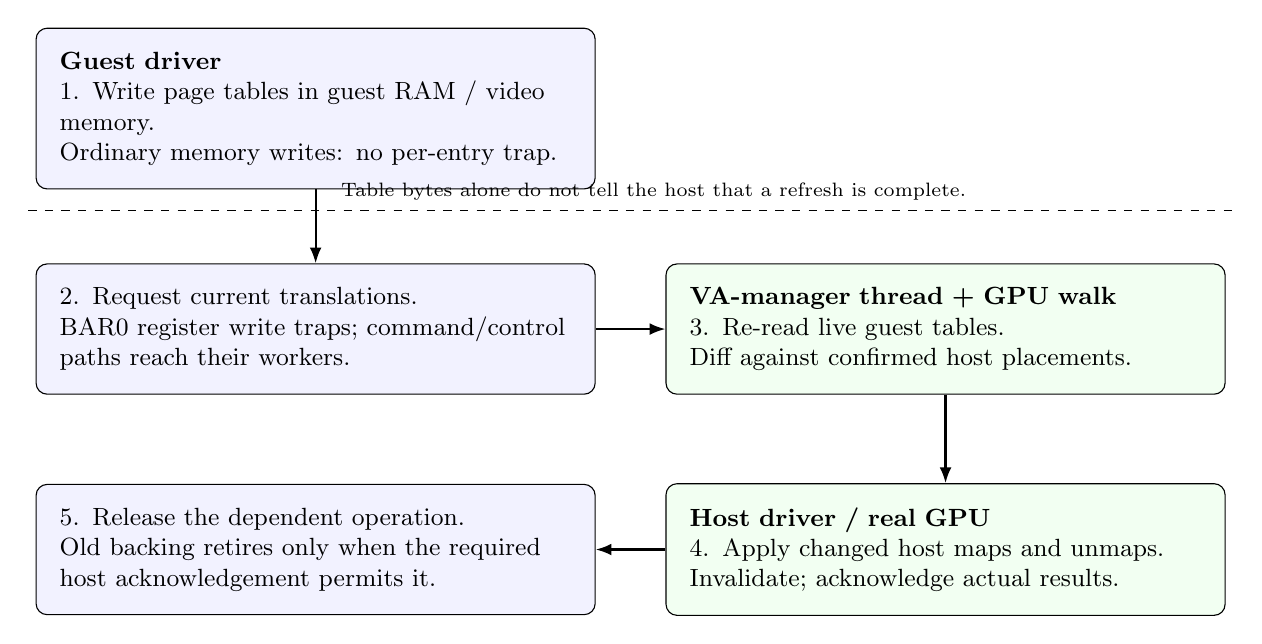
\begin{tikzpicture}[font=\small,
  box/.style={draw,rounded corners,align=left,text width=65mm,inner sep=3mm},
  flow/.style={-{Latex[length=2mm]},thick}]
\node[box,fill=blue!5] (guest) at (0,0)
  {\textbf{Guest driver}\\1. Write page tables in guest RAM / video memory.\\
   Ordinary memory writes: no per-entry trap.};
\node[box,fill=blue!5] (barrier) at (0,-2.8)
  {2. Request current translations.\\BAR0 register write traps; command/control paths
   reach their workers.};
\node[box,fill=green!5] (walk) at (8,-2.8)
  {\textbf{VA-manager thread + GPU walk}\\3. Re-read live guest tables.\\
   Diff against confirmed host placements.};
\node[box,fill=green!5] (host) at (8,-5.6)
  {\textbf{Host driver / real GPU}\\4. Apply changed host maps and unmaps.\\
   Invalidate; acknowledge actual results.};
\node[box,fill=blue!5] (dependent) at (0,-5.6)
  {5. Release the dependent operation.\\Old backing retires only when the required
   host acknowledgement permits it.};
\draw[flow] (guest) -- (barrier);
\draw[flow] (barrier) -- (walk);
\draw[flow] (walk) -- (host);
\draw[flow] (host) -- (dependent);
\draw[dashed] (-3.65,-1.3) -- (11.65,-1.3);
\node[anchor=west,font=\scriptsize] at (0.2,-1.05)
  {Table bytes alone do not tell the host that a refresh is complete.};
\end{tikzpicture}
\caption{The missing update path. Acknowledging step 2 before step 4 needs another way to
  prevent stale access; it is not justified by recording the request.\src{architecture}
  \src{translated}\src{latency}}
\label{fig:mapping-path}
\end{figure}


\doc A refused map can leave an address absent and therefore faulting. A refused unmap can
leave old host backing reachable, which is a different risk. The project's rules permit
acknowledging the former absence but do not generally permit pretending the latter retirement
succeeded. The early-acknowledgement alternative is therefore a real design question: it would
need fault/replay or another way to prevent stale access.\src{rulings}\src{applycode}

\subsection{Who manages the resources?}

\doc RM means \emph{resource manager}. The driver allocates objects for memory, address spaces
and channels, then names them with handles. A handle is an object name, not a physical address
or an access right by itself. On the guest side, the CPU driver speaks to firmware on the GPU
System Processor, or GSP. Kayfabe plays that firmware-facing peer, including boot, message
queues and replies, then independently asks the real host resource manager for resources.
It does not run NVIDIA firmware inside the emulated device.\src{architecture}\src{gspcode}

A page-directory base is the root used to find an address space's tables. The space can outlive
that particular root; a recycled root address must not silently identify a new object as the
old one. \emph{Mirror} means constructing host mappings from the guest's declared mappings,
not handing hostile guest tables directly to the real GPU.\src{architecture}\src{memcode}

\subsection{What a channel submits}

A \emph{channel} is an ordered execution context for an engine. A copy engine moves or fills
memory; graphics, compute and video engines perform other work. A timeslice group (TSG) groups
related channels for scheduling. Preserving each stream's bytes does not by itself preserve
its group or shared context.\src{kinds}\src{tsgcode}

A channel's \emph{GPFIFO} is a ring of references to command buffers, called pushbuffers.
A descriptor gives an address and length; the pointed-to buffer contains method packets and
arguments for an engine object. Packets can span descriptors. A software relay that inspects
commands must preserve packet state across those boundaries. A \emph{GP reference} is one
such command-buffer descriptor, not the bytes of the commands.\src{relaydesign}\src{turncode}

Each channel also has shared producer/consumer state, called USERD. The driver appends ring
entries, publishes its write index, GP\_PUT, and rings a \emph{doorbell}: a register notification
to inspect work. The GPU fetch unit advances GP\_GET as it reads entries. GET therefore means
``fetched'', not ``finished''. Commands behind a dependency may remain unexecuted after their
reference was fetched. A \emph{token} selects a channel route when a doorbell is rung; the
write does not prove which guest process sent it.\src{eventloop}\src{trapcode}

\subsection{Dependencies, completion and Windows recovery}

A \emph{semaphore} is a memory value used for dependency ordering: one operation releases a
value and another waits for it. A processed marker witnesses that execution crossed a chosen
point. A \emph{non-stall interrupt} invites software to inspect completion state; it is not
itself a per-packet completion receipt. Host notifications can be engine-wide.
\src{eventloop}\src{kinds}\src{faq}

\doc WDDM, the Windows Display Driver Model, schedules GPU tasks and handles recovery.
Microsoft documents a default two-second preemption wait. On a detected timeout Windows
attempts recovery; a recovered display can report that the driver stopped responding, while
applications may need to recreate their device. Engine and adapter recovery have different
scope. A reported 2.43-second host operation is not enough to prove which timeout occurred:
the scheduler's request time and the affected task must be identified.\src{mskeys}
\src{msrecovery}\src{walknarrow}

An \emph{Xid} is a host NVIDIA error record; Windows adapter Code 43 is an adapter status;
events 153 and 4101 are guest log observations used by the test records. They are different
observation domains, not names for one causal defect. A test must correlate them by time and
lifetime rather than treating one quiet counter as proof of health.\src{winmatrix}\src{faq}

\subsection{Sparse memory is a third state}

\doc A backed mapping points to real storage. A plain-invalid address faults. A sparse
mapping intentionally has no backing while absorbing writes and returning zeros on reads.
The selective sparse-mapping experiment tries to preserve that distinction; turning every
unmapped address sparse would also swallow accesses that should fault. Its finite reservation
budget and fallback can therefore affect compatibility as well as resource cost.
\src{sparse}\src{budget}

\doc UVM means unified virtual memory. Some managed-memory accesses need a page supplied on
first touch and the access replayed. Mirroring mappings already present does not deliver that
fault/replay service. This matters both for the remaining application failures and for the
proposal to acknowledge a mapping barrier early.\src{uvmdesign}\src{status}

\subsection{Three kinds of execution, three meanings of permission}

\doc Kayfabe calls ordinary guest-user execution \emph{Passthrough channels}; this is not VFIO
assignment of the whole GPU. Their host twins execute commands under GPU USER privilege in
restricted host address spaces. \emph{Translated channels} serve guest-kernel work by rewriting
addresses into an emulator-owned privileged space. \emph{Emulated channels} perform work that
belongs entirely to the virtual device. Only the last kind completes wholly in software.
\src{kinds}\src{architecture}

GPU USER privilege limits commands on hardware. The host driver's non-privileged request
interface limits which host operations Kayfabe may ask for. A Unix UID controls host process
credentials. A source or benchmark that establishes one boundary does not establish the other
two, and none is a substitute for fault-containment tests.\src{security}\src{physevidence}
\begin{figure}[H]
\centering
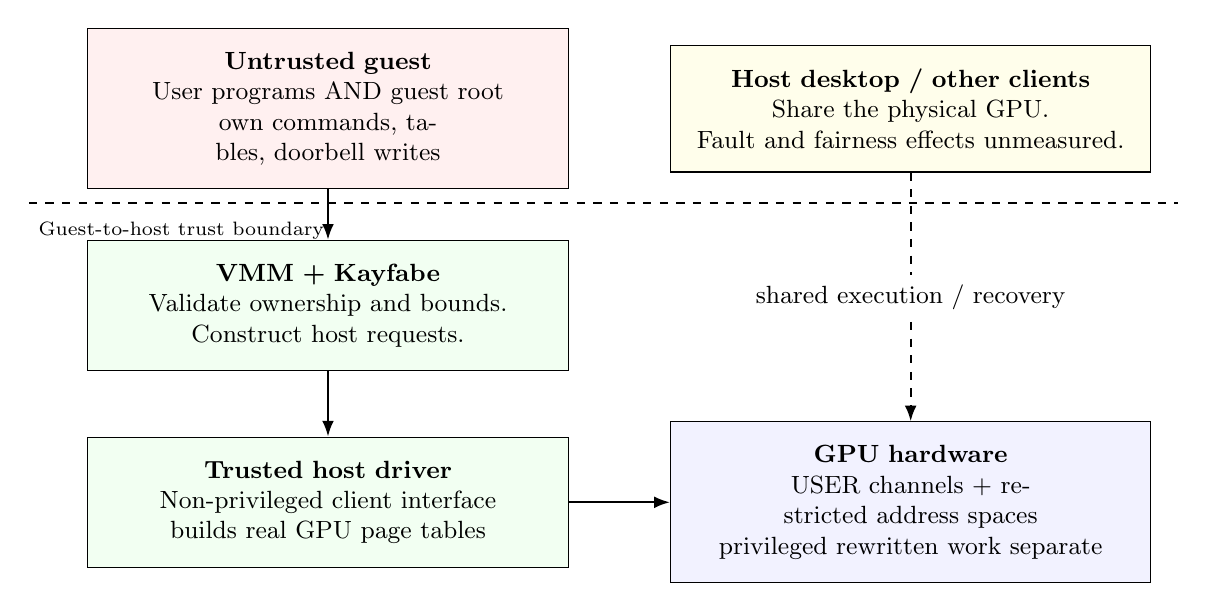
\begin{tikzpicture}[font=\small,
  box/.style={draw,align=center,text width=55mm,minimum height=12mm,inner sep=3mm},
  flow/.style={-{Latex[length=2mm]},thick}]
\node[box,fill=red!6] (guest) at (0,0)
  {\textbf{Untrusted guest}\\User programs AND guest root\\own commands, tables, doorbell writes};
\node[box,fill=green!5] (vmm) at (0,-2.5)
  {\textbf{VMM + Kayfabe}\\Validate ownership and bounds.\\Construct host requests.};
\node[box,fill=green!5] (driver) at (0,-5)
  {\textbf{Trusted host driver}\\Non-privileged client interface\\builds real GPU page tables};
\node[box,fill=blue!5] (gpu) at (7.4,-5)
  {\textbf{GPU hardware}\\USER channels + restricted address spaces\\
   privileged rewritten work separate};
\node[box,fill=yellow!8] (host) at (7.4,0)
  {\textbf{Host desktop / other clients}\\Share the physical GPU.\\
   Fault and fairness effects unmeasured.};
\draw[flow] (guest) -- (vmm);
\draw[flow] (vmm) -- (driver);
\draw[flow] (driver) -- (gpu);
\draw[flow,dashed] (host) -- node[fill=white,align=center,text width=44mm]
  {shared execution / recovery} (gpu);
\draw[dashed,thick] (-3.8,-1.2) -- (10.8,-1.2);
\node[anchor=west,font=\scriptsize] at (-3.8,-1.55) {Guest-to-host trust boundary};
\end{tikzpicture}
\caption{Three permission systems: host request permissions, GPU channel privilege and Unix
  credentials. Host address isolation alone does not prove host-desktop fault containment.
  \src{security}\src{rulings}}
\label{fig:trust}
\end{figure}


\section{Architecture v3: where authority and progress live}
\label{sec:architecture}

The implementation baseline is the cover revision. CODE statements below name implementation
paths; DOC statements describe requirements or published designs. The test descriptions name
what could exercise an invariant. Unless a dated result is given in Section~\ref{sec:results},
their pass state at this baseline is UNVERIFIED: no product test was run for this edition.

\subsection{Planes and traps}

\doc The product is the \code{kf-*} tree linked into the VMM process. A BAR0 write
records demand through bounded token and ring state. Workers service channel demand; a
register drainer services privileged register operations. BAR1 and BAR2 memory accesses do not
trap. There is no separate isolate process or product IPC plane. Confinement applies to the
whole hypervisor process.\src{architecture}\src{corecode}\src{trapcode}

\attack{No host mapping or blocking operation runs on a vCPU or under a lock it takes.}
{The trap crate's unit tests, core composition tests and source restrictions constrain the
reachable trap path. Hardware trap timing checks a separate latency property.\src{trapcode}}
{A nonblocking-looking call can acquire a lock held by slow host work. A mock host that never
blocks cannot demonstrate the production lock discipline. The old paper records that failure
mode; the restriction must be checked transitively.\src{old}}

\subsection{Hostile input and authored operations}

\doc Guest root and guest userspace are untrusted. Host memory operations are constructed
from admitted ownership, extent, permission and kind information; guest control messages are
not replayed to the host. Host GPU facts come from unprivileged queries or generated open
interfaces. This is the intended authority boundary, with the host driver and GPU trusted.
\src{security}\src{architecture}\src{hostcode}

\attack{No guest-chosen raw address or privilege request creates new host authority.}
{Hostile range/ownership tests, channel privilege tests and the physical-operand hardware
oracle exercise different pieces of this claim.\src{security}\src{physevidence}}
{Checking a decoder cannot establish that every caller uses it. A guest-declared OS identity
also cannot prove a safe mapping scope. Whole-path reachability and multiple-VM fault effects
remain separate review obligations.\src{rulings}\src{security}}

\subsection{Derive, never capture}

\doc The architecture prefers facts read from the host's own unprivileged interface,
computed virtual-device state and rules generated from pinned open headers. A device identity
is not permission to copy another die's answer. Request validation and field-level virtual
support still apply when an answer comes from the host. Published measured exceptions belong
to exact die/driver coverage, not an invisible default table.\src{architecture}\src{constants}

\attack{Every guest-visible field has a source and a defined unsupported case; an unknown die
never silently inherits a neighbour's observation.}
{The constants strategy requires source tags, derivation oracles, wrong-answer mutations and
same-die native acceptance. It explicitly separates the implemented baseline from table
consumers on branches.\src{constants}\src{provenance}}
{A source tag proves provenance only if its source actually supports the field. A boot that
never exercises an optional feature cannot verify that feature, and agreement between a few
dies is not a mechanism for a family rule.\src{constants}}

\subsection{Seven axes, not one compatibility version}

\doc The design separates guest kernel, guest driver, host driver, GPU architecture,
GPU die, VMM and guest OS. An architecture supplies family mechanisms; a die supplies actual
inventory and capability facts. The guest ABI controls decoding; the host ABI controls authored
calls. The VMM supplies memory, interrupts and lifecycle events. These are distinct axes even
when a test holds several fixed.\src{design}\src{constants}\src{driverdesign}

\begin{center}\small
\begin{tabularx}{\textwidth}{@{}lXX@{}}
\toprule Axis & Boundary to inspect & Counterexample worth testing \\
\midrule
Guest kernel & DMA addressing / virtual IOMMU & IOVA mistaken for guest physical address \\
Guest driver & versioned decode / accepted replies & layout changes within a branch \\
Host driver & authored RM ABI & successful syscall with failed in-band status \\
Architecture & class / register / MMU family & different engine or boot protocol \\
Die & runtime facts / measured exceptions & floor-swept or unmeasured die \\
VMM & memory, IRQ, reset adapter & reset origin or wake semantics differ \\
Guest OS & driver protocol and scheduling & Windows registration / recovery path \\
\bottomrule
\end{tabularx}
\end{center}
The counterexamples are proposed attacks, not claims that each has occurred at the baseline.
A matrix that changes one axis at a time is evidence for those cells, not the full Cartesian
product.\src{driverdesign}\src{constants}

\attack{Guest and host ABI choices remain independent, and OS or VMM identity never grants
extra memory authority.}
{The driver matrix tests named host/guest cells; versioned decoder oracles check layouts.
Portability beyond QEMU and x86-64 still needs real adapter evidence.\src{driverdesign}
\src{requirements}}
{A layout may change within a driver branch, and a cross-build cannot exercise mapping,
interrupt or reset semantics. Passing one axis with the others fixed is not the full grid.}

\subsection{Crate map and the frozen predecessor}

\doc The following is a functional map from \code{ARCHITECTURE.md}, not a generated
claim about every dependency edge.\src{architecture}
\begin{center}\small
\begin{tabularx}{\textwidth}{@{}p{42mm}X@{}}
\toprule Crates & Responsibility \\
\midrule
\code{kf-trap}, \code{kf-core} & bounded demand publication and plane composition \\
\code{kf-gsp}, \code{kf-rm} & firmware-facing protocol and resource-manager model \\
\code{kf-chip}, \code{kf-abi} & host facts, family rules and versioned generated layouts \\
\code{kf-host} & one in-process host RM session and authored verbs \\
\code{kf-mem}, \code{kf-cuda} & backing store, VA manager, GPU walk and diff protocol \\
\code{kf-chan} & channel birth, translated work, relay and completions \\
\code{kf-qemu} + C device & QEMU memory, lifecycle, interrupt and device adapter \\
\code{kf-disp}, \code{kf-broker} & emulated display and VMM-neutral broker protocol \\
\code{kf-oprom}, \code{kf-gop-image} & generated boot-display container and build \\
\code{kf-harness} & real-GPU tests without QEMU \\
\code{kf-census}, \code{kf-crec}, \code{kf-trace} & offline tools and historical oracles \\
\code{kf-arch}, \code{kf-linux-raw}, \code{kf-util} & vocabulary, audited OS calls, utilities \\
\bottomrule
\end{tabularx}
\end{center}

\doc The older \code{kayfabe-*} crates remain frozen; the raw-client grader depends on
part of that tree. Product \code{kf-*} crates do not depend on it. Unsafe code is confined to
named adapter crates and \code{*_unsafe.rs} files. A crate inventory is a source-level fact;
it says nothing about whether a feature has a production caller.\src{rules}\src{architecture}

\attack{Product crates retain their dependency and unsafe boundaries; the frozen grader tree
never becomes a hidden product dependency.}
{Workspace manifests and CI boundary checks enforce structural restrictions. Reached-path
oracles and real adapter tests address behaviour separately.\src{rules}\src{architecture}}
{A legal dependency graph can still contain an unused implementation or a production-only
blocking path. Source structure does not establish reachability or hardware correctness.}

\subsection{Channel kinds and the meaning of completion}

\doc Passthrough creates a host twin for user work and lets the real engine execute its
commands. Translated channels rewrite kernel copy work into an owned address window and submit
it to the real engine. Emulated channels execute only work whose meaning belongs entirely to
the VMM. The three kinds differ in authority and completion, not simply speed.\src{kinds}

\attack{No CPU executor substitutes for GPU work; no completion is forged for work submitted
to hardware.}
{The channel suites and real-engine gates check actual execution, content and notification.
The translated-plane design separates address arithmetic from execution.\src{translated}}
{An application can report success without checking its GPU error or result. A harness must
validate the output and completion path, not merely the process exit.\src{status}}

\subsection{Memory store and VA manager}

\doc Guest video memory is one host allocation with offsets corresponding to guest
framebuffer offsets. Guest system memory comes from the VMM's shared backing. A GPU walk
reads guest tables and diffs them against confirmed host placements. Host maps/unmaps apply
the changes, invalidate, and acknowledge runs. A refused map remains a difference.
The committed-placement record is not an adopted guest page table.\src{architecture}
\src{diffcode}\src{memcode}

\attack{Only acknowledged host placements become committed state. Old backing remains owned
until the relevant invalidation acknowledges its retirement.}
{The diff model, apply tests and hardware walk gate compare emitted runs, acknowledgements
and resulting translations. The retirement experiment adds explicit delayed-free tests.
\src{diffcode}\src{applycode}\src{retirementpr}}
{A software model can assume host RM ordering that hardware does not provide. Table roots,
shared subtrees, root withdrawal and failed host invalidation require separate schedules.
Whole-space scanning is not equivalent to remapping every unchanged leaf.\src{latency}}

\subsection{Mirrored scheduling groups}

\readcode Host group/member construction preserves a guest TSG grouping, and twin lifetime follows
the trusted object model.
The late-joiner design documents why a newly added channel cannot silently miss earlier
scheduling state. Address-space mirroring and TSG mirroring are separate concerns: preserving
one does not prove the other.\src{tsgcode}\src{latejoin}\src{kinds}

\attack{Channels in one guest scheduling group retain the corresponding host grouping and
required state as members arrive and leave.}
{Grouping tests and the video-engine validation exercise group creation and related channel
use.\src{tsgcode}\src{video}}
{A test with all channels present at initial configuration misses late arrival. Reused handles
and reset generations can make a correct group lookup refer to the wrong life.\src{latejoin}}

\subsection{User-ring lifecycle: Scan, Pointer and Window}

\doc A registration is a guest request that arms a later software action in its
command stream; that action can move the ring source. Windows user-work can therefore require
software intervention around registration and ring
migration. In Scan mode the worker inspects command packets. Pointer mode forwards admitted
GP references without reading the pushbuffer. Window mode restores scanning across the
registration boundary. An anchor is an observed producer position selected as that boundary.
The clean anchor must have been observed before the registration reply;
a later convenient cursor cannot retroactively establish that boundary.\src{lifecycle}

\attack{Doorbell-covered entries appear once, in order and bit-exact; Pointer reads no
pushbuffer; a validated descriptor is the snapshot actually published.}
{Real-turn model, property and threaded stress suites cover mode transitions, ring migration,
packet continuation, poisoned bytes above PUT and registration at different positions.
\src{lifecycle}\src{turncode}}
{Finite model schedules can omit a real host lock holder, DMA ordering or guest mutation.
A normal-user experiment cannot certify a hostile user that rewrites its own memory.
The boundary remains native USER privilege plus admitted mappings.\src{rulings}}
\begin{figure}[H]
\centering
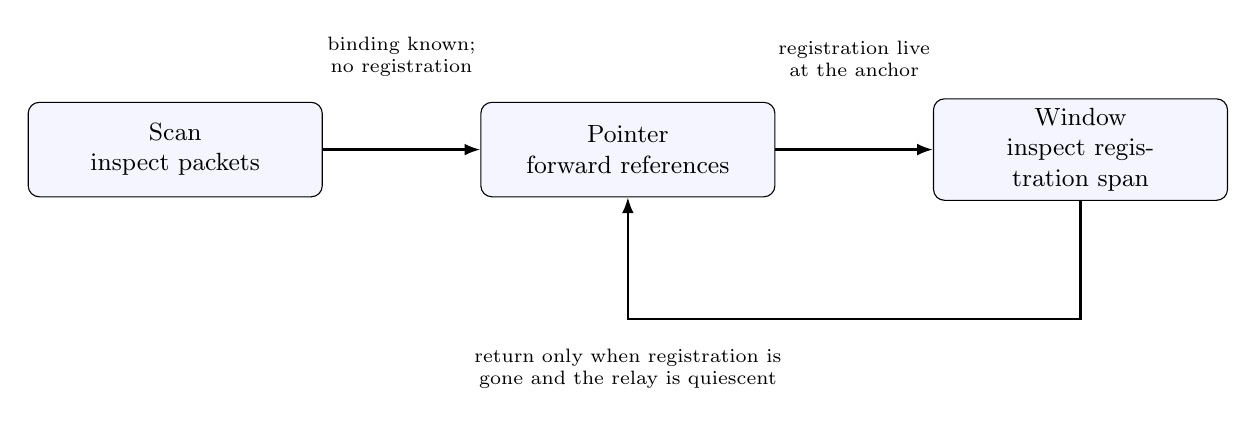
\begin{tikzpicture}[node distance=20mm]
\node[concept] (scan) {Scan\\inspect packets};
\node[concept,right=of scan] (pointer) {Pointer\\forward references};
\node[concept,right=of pointer] (window) {Window\\inspect registration span};
\draw[flow] (scan) -- node[above=8mm,align=center,font=\scriptsize,text width=32mm]
  {binding known; no registration} (pointer);
\draw[flow] (pointer) -- node[above=8mm,align=center,font=\scriptsize,text width=32mm]
  {registration live at the anchor} (window);
\draw[flow] (window.south) -- ++(0,-15mm) -| (pointer.south);
\node[below=18mm of pointer,align=center,font=\scriptsize,text width=60mm]
  {return only when registration is gone and the relay is quiescent};
\end{tikzpicture}
\caption{Main lifecycle path; direct Scan-to-Window and teardown edges are omitted.
  Registration and packet-boundary rules govern each transition.\src{lifecycle}}
\label{fig:lifecycle}
\end{figure}


\subsection{Lazy observation: a stale view must only delay}

\readcode Pointer mode caches a previously loaded PUT within the same ring generation and
reduces private USERD observations. Scan and Window remain fresh. Low credits, waits, split
segments and a full guest ring force observations. A stale GET may reduce available credit;
it must never increase credit or release a marker gate early. Mode changes and migration
invalidate cached state.\src{lifecycle}\src{lazycode}

\attack{No idle decision relies on cached PUT, and no stale observation is the sole missing
wake for a wait that can already be satisfied.}
{The lazy-turn suites compare forwarding identity with observation enabled and disabled,
exercise small rings, and test forced observations and generation changes.\src{lifecycle}}
{A counter of fewer reads is not proof of liveness. Combined performance arms cannot attribute
speed to each optimisation separately. Hardware completion and holder-release timing remain
outside the pure predicate model.\src{lifecycle}}

\subsection{Relay, handoff and interrupts}

\readcode The relay has explicit progress obligations. If a storage, row or page-table holder
prevents progress, release must arrange another attempt; repeatedly trying a busy lock is not
an event-delivery proof. The baseline includes the relay handoff fix cited by the README and
a later merged lost-wake correction. Experimental split-latency instrumentation keeps that
relay design rather than introducing an attempt limit.\src{readme}\src{turncode}\src{latency}

\attack{Registering a waiter concurrently with completion or lock release cannot lose the
last wake. An interrupt invites a check; it does not manufacture a completed fence.}
{Relay interleaving tests, completion tests and the live regressions cited in the README
exercise parts of this claim. The later probe experiment explicitly diagnoses missing wakes.
\src{readme}\src{probepr}}
{Host events are GPU-wide, so an interrupt can be unrelated to this channel. Observing a marker
late does not timestamp when the GPU wrote it. A worker busy elsewhere can delay observation
without a lost physical event.\src{faq}\src{latency}}

\subsection{Display and the broker}

\doc An emulated display engine accepts the stock driver's display protocol; a separate
broker presents owned frame copies and handles input. The display contract requires guest flips to
complete according to guest semantics while copies select the newest frame independently.
The broker owns cursor composition, including inversion. Its absence or silence must not
freeze guest display progress.\src{architecture}\src{display}\src{rulings}

\attack{Guest flip completion is independent of a stalled viewer; frames and credits remain
bounded; the broker never receives arbitrary guest memory as an owned frame.}
{Display engine tests, plane-output oracles, socket simulations and pacing models exercise
flip order, slow brokers and pixel formats.\src{display}\src{planes}\src{pacing}}
{A fake broker cannot establish compositor, DMA-buffer or colour behaviour on every desktop.
Correct pixels do not prove correct flip latency, and a correct cursor does not prove safe
frame ownership.\src{pacing}\src{security}}

\section{What the evidence establishes}
\label{sec:results}

\subsection{A result belongs to a cell and a revision}

\readcode The status-detail document warns that much of its main body is September history.
The README and newer per-topic records add Windows, display and relay results. This paper
therefore does not copy a historical heading such as ``Windows: research only'' into a current
support claim. Conversely, a later source audit does not rerun an earlier hardware test.
The following table deliberately retains the recorded revisions.\src{status}\src{readme}

\begin{center}\small
\begin{tabularx}{\textwidth}{@{}p{25mm}p{27mm}X@{}}
\toprule Cell & Revision & Recorded scope; repetition limit \\
\midrule
Linux / TU116 & \code{1915bd71} & Gates 9/9, bare and thin 30/30; one recorded merge-bar
campaign. Ladder at \code{a295e2ce}, described as the same code. No timing spread claimed.
\src{turing} \\
Linux / AD104 workstation & \code{fc2dadc4} & Gates 9/9, bare and thin 30/30; ladder
4/4 at \code{d40dafbf}. Distinct checkout revisions are preserved.\src{families} \\
Linux / GB205 & \code{d40dafbf} & Gates 9/9, bare and thin 30/30, ladder 4/4.
One recorded cell, not a Windows pass.\src{families} \\
Linux / GA104 & \code{714ec29d3} & Host and guest 595.91.07; gates 9/9 plus gate 10,
bare and thin 30/30, one box/cell.\src{requirements}\src{sweep} \\
Windows / AD104 desktop & \code{eb9f2aa3} & Stock 580.88 application matrix; later
relay session at \code{89fc8a222}. Completion, recovery and output grades differ by app.
No full-matrix pass at the paper baseline is asserted.\src{readme}\src{winmatrix} \\
\bottomrule
\end{tabularx}
\end{center}

\measured The family records above are dated 2026-09-30; the GA104 record is dated
2026-10-24. Pass counts enumerate tests or arms, not independent boots of the entire workload.
A 30/30 thin suite boots separate arms; it is not a thirty-boot confidence interval for a
multi-application desktop. The Linux family campaigns used nested rented hosts and open
580.159.04 drivers unless the cell says otherwise.\src{turing}\src{families}\src{sweep}

\readcode The public requirements list additional earlier Linux runs on GA106, GA102,
AD106 and GB203, and the README mentions an AD102 Linux guest with driver 590. Windows desktops
on AD106 and AD103 used a borrowed display page. The requirements explicitly say that no single
current per-die table is documented. This is evidence fragmentation, not permission to call
all neighbouring dies supported. Hopper and datacentre families remain source-derived or
refused cases, not hardware qualifications.\src{requirements}\src{readme}

\subsection{Correctness results and their sample units}

\measured The recorded Linux application matrix reports 61/65 passing applications and six
stream probes, with output comparisons to the same host; its source is an earlier GA106
campaign, not the paper baseline. The four remaining failures need managed-memory demand
paging. The record of 100 sequential processes applies to one persistence-mode boot. These
are useful workload and lifetime samples, but neither is a soak distribution.\src{status}
\src{apps}\src{readme}

\measured The headless graphics record reports 38/38 items, including 31 byte-identical
outputs, at \code{d06833f0} on a GA104 box. The video lane reports byte-identical encode/decode
outputs on a GA106. These compare content, which is stronger than a renderer name; they do
not cover every display mode, all video families or later revisions.\src{status}\src{video}

\readcode The driver matrix varies host and guest independently. Several guest versions
passed a CUDA ladder against a fixed host, and several hosts passed the gates, thin suite and
ladder against a fixed guest. The public guide preserves the versions and revisions and warns
that the raw 30-arm suite is graded for 580.x guests. A decoder's support range and a tested
application range are different sets.\src{requirements}\src{driverdesign}

\subsection{A performance row with actual spread}

\measured At device revision \code{e5ff45ff}, the AMD EPYC 7452 nested host with RTX 3060
and 580.159.04 ran eager Qwen2-0.5B decoding. For 512-token warm decode, the summary gives
\textbf{12.62 tokens/s [12.40, 12.94], $n=3$} in the guest and
\textbf{43.98 [43.59, 44.63], $n=3$} on the host, ratio \textbf{0.287}.
These are the table's reported aggregates and ranges, not a new estimate or confidence
interval. The associated text-equality checks matter separately from throughput.
\src{llmmethod}\src{llmdata}

\measured The Windows performance summary, 2026-10-17, records three experimental
Direct3D 11 Heaven runs at \code{134dcb54}: \textbf{299.1, 296.5 and 299.2 fps}
with scan-off and lazy observation together, 1920$\times$1080, Ultra, 260-second windows,
stock 580.88 guest on the owner's AD104 host with 595.91.07. Its production-path samples at
other listed revisions are slower. The record itself says these experiments were not a
safe integrated lifecycle qualification and did not have an application matrix. Their
combined gain cannot be assigned to just one optimisation.\src{winperf}

\inferred These examples support two narrower conclusions: large batches and small launches
need separate measurements, and a fast renderer can coexist with a correctness or latency
problem under mixed use. They do not establish a universal ``virtualisation overhead'' number.
Nested versus non-nested execution, host load, guest workload and baseline revision all change
the denominator.\src{linuxperf}\src{winperf}

\subsection{The Worker GPU gate: useful, unattested and owner-controlled}

\readcode GitHub requests a check through a Cloudflare Worker. A Durable Object ledger
reserves liability, tracks owned instances, deadlines and spending, and coordinates cleanup.
The provider account key stays in the Worker. Identity checks bind the workflow, owner
triggering actor, signed run attempt and tested SHA. A scoped box capability can report only
within its run contract. Cloudflare Access reduces noise; it is not the content-approval
boundary.\src{broker}\src{threat}

\readcode At the baseline's contributor policy, ordinary PRs target \code{next}; the GPU
check belongs on the exact final \code{next} to \code{master} batch. The policy states CI is
required on next and CI plus \code{gpu-vast} on master. This is the recorded policy, not an
audit of live GitHub ruleset settings. Older triage or handoff statements about required
checks are historical.\src{rules}

\attack{Only the owner-approved SHA rents within the configured policy, and cleanup acts on
ledger-owned instances.}
{Broker unit/runtime tests and recorded provider campaigns exercise identity, accounting,
results, retries and teardown. A real runtime matters because Node fakes cannot reproduce
all Worker fetch behaviour.\src{threat}\src{broker}}
{The rented machine and its operator can lie. A valid callback authenticates the run capability,
not honest GPU execution. A PASS is a regression tripwire, not release provenance, an
attestation or a security audit. A missed cron or failed provider deletion can also outlive
an internal deadline.\src{broker}\src{threat}}

\clearpage
\section{The uncomfortable part}
\label{sec:uncomfortable}

The following is the research ledger, not a collection of release promises. It distinguishes
fixed defects, competing explanations, experimental code and unrun acceptance tests. The
open-PR inventory at the end preserves the publication snapshot; an open PR is not evidence
that all of its changes are absent from the baseline.

\subsection{The multi-application stall: start with the dependency, not its name}

\readcode The October investigation asks why Windows applications can stall or recover while
individual workloads run well. The later mapping experiments use the Enscape arm of the
SPECviewperf workload. This paper discusses the failure and its timings; it publishes no
SPEC scores, viewset results or proprietary workload images. The experimental mapping line
is distinct from the baseline's earlier relay fixes.\src{admission}\src{rmcost}\src{latency}

A useful causal chain has separate stages: Windows queues work; the relay observes demand;
it publishes host work; the GPU processes a covering marker; host software observes that
marker; the interrupt path notifies the guest; the guest scheduler observes progress. A
silence at the end does not locate the missing or late step. The proposed diagnostic contract
keeps these stages separate and explicitly refuses to identify a private host publication
with a Windows packet without evidence.\src{latency}\src{walknarrow}
\begin{figure}[htbp]
\centering
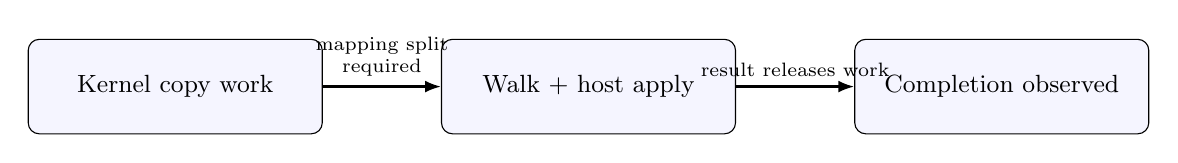
\begin{tikzpicture}[node distance=15mm]
\node[concept] (a) {Kernel copy work};
\node[concept,right=of a] (b) {Walk + host apply};
\node[concept,right=of b] (c) {Completion observed};
\draw[flow] (a) -- node[above,align=center,font=\scriptsize,text width=25mm] {mapping split
  required} (b);
\draw[flow] (b) -- node[above,align=center,font=\scriptsize,text width=25mm] {result releases work}
  (c);
\end{tikzpicture}
\caption{A serial dependency can resemble a missing interrupt; clocks and packet identity decide.}
\label{fig:stall}
\end{figure}


\subsection{Timeline: defects that really existed, and explanations that did not survive}

\begin{enumerate}[itemsep=0.7em]
\item \readcode The October 9 invalidate incident left a guest trigger incomplete:
  run 223 counted 3,138 invalidates and 3,137 clears. The owner ruling records a guest polling
  that trigger indefinitely. Clearing over absent guest leaves became a policy; refused
  host unmap or host invalidate was explicitly not covered by that exception. A later
  reservation-edge defect was Kayfabe's mapping failure, not invalid guest tables.
  These are documented predecessors, not proof of the later Enscape cause.\src{rulings}
\item \readcode The earlier USER-ring completion gate used GET as a witness. The event-loop
  record says hardware could fetch beyond a dependency before the dependent work ran.
  A tagged processed-reference marker replaced that proof. The attractive explanation
  ``GET passed it, so it executed'' was too strong.\src{eventloop}
\item \measured The README records an earlier relay-handoff campaign with 0 stalled pairs
  out of 26 after the fix, against 3 out of 12 before, plus a later Windows mixed-app session
  of more than fifteen minutes. These are the README's scoped reports at \code{89fc8a222};
  the paper does not claim a population-wide stall rate or transfer that result to the
  later sparse experiment.\src{readme}
\item \readcode A later Translated-slot contention defect consumed a wake while another
  thread held the channel slot. The token could return idle with no owner or future pump.
  The merged recovery retains the owed ring; behavioural tests demonstrated cases that
  source-shape guards had missed. Its design record also says a Turing run still had
  Windows reset storms after the narrow wake defect was fixed.\src{owed}
\item \readcode The first sparse-admission implementation cloned and restored the whole
  reservation tree on failure, returned an uncounted hard error for occupied coarse geometry,
  and could resend a failed acknowledgement on later walks. Local undo, explicit decline
  accounting and retry metadata addressed those software mechanisms. Their CPU tests
  were not an Enscape acceptance run.\src{admission}
\item \measured At sparse-admission revision \code{6d95870c7}, runs 7330 and 7350 showed
  reservation churn near the 8,192-block policy boundary. In run 7330, over approximately
  66 seconds, made objects rose by 241,584 and freed objects by 241,583. The record also
  reports a 1.94-second apply with roughly 59,000 reservation verbs. This refutes the
  simple explanation that every long apply must be one slow native call.\src{rmcost}
\item \measured That same record puts run 7330's first event 153 near the Enscape start
  while recent VA heartbeats were idle. Missing sparse coverage and declines coincided
  with onset. This argues against treating earlier reservation-churn latency as a complete
  account of that particular first reset. It does not prove missing coverage caused it.
  \inferred The hypotheses require separate interventions.\src{rmcost}
\item \readcode Later scope tests passed on the original gate while harvesting a published
  marker and writing GET back before the PUT admission gate. They falsify the narrow
  claim that this gate alone prevents completion observation. They do not falsify delayed
  worker scheduling, lock contention or a dependency before publication.\src{walknarrow}
\end{enumerate}

The timeline is deliberately non-monotone: a real lost wake, a throughput defect and a missing
mapping can all occur during one campaign. Finding the next defect does not retract a
previously demonstrated one, and fixing the previous one does not close the new case.

\subsection{What the later walks actually say}

\measured The public split-latency note attributes \textbf{297,495 of 318,747} walks in boot
7321 and \textbf{461,389 of 490,686} in boot 7391 to one privileged Translated copy-channel
token. These are roughly \textbf{93--94\%}, with one count pair per boot, not a sampled estimate
with a confidence interval. The note is a secondary report supplied to the implementation
review; this paper has not audited the raw host traces.\src{latency}

\measured The scope-narrowing note reports a \textbf{2.43-second apply} and a
\textbf{2.529-second completion gap} in boot 7391 at \code{64c50ad4}. With raised diagnostic
TDR thresholds, that Enscape arm reached its time limit without event 153. The note reports
completion intervals following walk ends in boot 7321. These observations support a
\emph{late rather than permanently lost} account for that arm; they are not a timeout-based
fix, a broad timing distribution, or a one-to-one packet-identity proof.\src{walknarrow}

\inferred A mostly serial channel that asks for a mapping split, waits for its result and
then issues the next request can produce one observed completion near each walk end. That is
consistent with the timing report. Identifying the Windows scheduling node with that exact
host channel still requires ticket-level correlation. Correlation of two periodic series is
not the missing identity.\src{latency}\src{walknarrow}

\readcode A split requests a fresh post-admission walk because releasing later work against
an earlier snapshot could expose stale translations. Same-target tickets admitted together
can share a walk; a request arriving during an active walk belongs to a later submission.
A channel that waits for each result before issuing the next request supplies nothing
concurrent to coalesce.\src{latency}

\textbf{Acceptance still absent from the cited record:} a full production-profile,
default-timeout, sparse-twin-enabled Windows boot that passes the failing mixed workload.
The software validation notes explicitly retain pending host acceptance and the default-OFF
sparse policy. A longer diagnostic timeout cannot fill that gap.\src{sparse}\src{budget}
\src{latency}

\subsection{How our explanation could be wrong}

\textbf{First fork: publication delay versus observation delay.} A packet can spend its time
waiting to be published, executing on hardware, or complete while the observing worker is
busy. The native marker has no GPU-write timestamp in the current diagnostic contract;
\code{marker_gpu_ns=None} is intentional. Publication-to-observed-marker therefore combines
execution and observation latency. Calling all of it ``GPU time'' would be false.
\src{latency}

\textbf{Second fork: CPU scope versus shared hardware.} A VM-wide admission gate can delay an
unrelated ring before publication. Narrowing it by trusted host mutation target removes that
particular dependency. It cannot remove shared engine scheduling, a global host RM lock, or
necessary same-target ordering. If the same stalls persist with unrelated holds removed,
that does not show the scope fix was inert; it shows the intervention did not isolate the
remaining bottleneck.\src{walknarrow}

\textbf{Third fork: trigger, victim and common cause.} A kernel copy channel can request most
walks while an application merely suffers from them. Alternatively, the application's
allocation pattern can cause both sparse work and scheduler distress. Per-channel walk
counts alone cannot distinguish those stories. The decisive observation needs request,
walk start, apply end, readiness, consumption, publication and notification in one life and
clock domain.\src{latency}

\textbf{Proposed falsifier, not a run result:} repeat the same workload and fixed image with
native publication/marker/vector histories and guest event tracing. Include a diagnostic
\code{TdrDelay=60} arm only as an observation window, alongside unchanged default thresholds.
If long completion gaps occur without a corresponding pre-publication split hold, reopen
relay/observation and GPU scheduling explanations. If changing sparse coverage alone changes
onset while latency remains unchanged, prioritise the semantic mapping hypothesis. Record
missing coverage and incomplete timestamps rather than dropping those samples.

\subsection{Sparse backing: semantic fidelity has a resource cost}

\readcode A sparse guest page is not the same as an invalid unmapped address. The selective
sparse-twin experiment exists to reproduce that distinction using host reservation objects.
It stays default OFF. A native micro-oracle can show that the sparse state changes a fault
outcome without proving a long-lived Windows desktop remains correct.\src{sparse}\src{sparsepr}

\readcode The newer policy scales finite per-space and per-session object budgets from the
configured guest framebuffer and counts missing coverage separately from cumulative declines.
Its interval tracker uses an explicit conservative upper bound on overflow; it must not turn
unknown missing coverage into a zero gauge. A permanently excluded host-owned window remains
excluded rather than repeatedly retried. These choices prefer faulting to inventing zero-filled
backing or taking ownership of a host placement.\src{budget}

\inferred This is a design tradeoff that deserves an unfriendly name: the fallback can be
closed for host authority while still incompatible with a guest that needs sparse semantics.
A finite cap protects the host; it does not make the guest's request disappear. The acceptance
question is whether supported workloads stay within the defined mode, not whether a counter
has an appealing value.\src{budget}\src{rulings}

\subsection{Soft budgets are not deadlines}

\readcode The sparse layout allowance limits the work that may \emph{start} in one slice.
Already started replacements must finish or repair their original ownership. An individual
native RM call is not software-preemptible. Ordinary map/unmap, invalidation, retirement and
full teardown are not all covered by the optional-layout allowance.\src{rmcost}\src{budget}

\measured A later CPU simulation with 120-ms releases required 240 ms for release and
mandatory repair, even after two budget bypasses were fixed. That result explicitly disproves
a universal 110-ms expectation. The original assertion of at most one replacement overshoot
was false for error cleanup that started additional work without checking the slice.
These are simulated timings at the scope-repair checkpoint, not a hardware guarantee.
\src{walknarrow}

\readcode The latest experimental continuation defers optional geometry until mandatory
split results and wakes are released, rotates among target identities and stops between
native verbs when a new split arrives. Mandatory repair still completes. Under continuous
mandatory work, optional coverage may remain unhonoured; it is counted rather than hidden.
No hard total-apply deadline or Windows cure is established.\src{latency}

\subsection{Mirrors: retiring memory is an ordering protocol}

\readcode A mirrored address space contains host placements, not merely a dictionary of guest
addresses. The retirement PR delays freeing old backing until invalidation acknowledges that
hardware can no longer use the old translation. A failed invalidate retains ownership.
Its original proposal also keeps explicit unresolved scope tests rather than claiming a
per-range gate exists.\src{retirementpr}\src{walkscope}

\inferred A mirror can be correct after every completed refresh and still produce excessive
latency during a refresh. Conversely, narrowing an admission gate can be fast and wrong if it
releases a source whose mapping is still changing. The experimental target-scoping argument
is about the host object actually mutated, not an assumption that distinct guest roots never
share table pages. Unknown/global requests retain conservative holds.\src{walknarrow}

The remaining fork is per-range certification: can unchanged source spans continue through an
own-space refresh while changed spans permit only old, new or fault outcomes? The latest note
marks that as design work. It needs a bounded change history, root-generation handling,
overflow fallback and publication revalidation; a per-space flag alone is not that protocol.
\src{latency}\src{walknarrow}

\subsection{Pointer mode and lazy observation: the proof costs more than the optimisation}

\readcode Pointer mode exists because repeatedly reading command bytes costs CPU time even
when hardware can safely read the guest's own admitted commands. Registration and migration
still require scanning boundaries. A window anchor is a fact about what was observed before
a reply; retrospectively choosing the current PUT would weaken the proof. The lifecycle
record corrects earlier boundary and mode-scope claims in place.\src{lifecycle}

\readcode Lazy observation additionally makes the guest-visible GET lag. The code compensates
with fresh observations on waits, low credits, split segments, full-ring pressure and mode
changes. Its argument is that staleness can only reduce credit or delay a gate, never create
progress. The small-ring bound matters because a large benchmark ring can hide guest
backpressure.\src{lifecycle}\src{lazycode}

\inferred These mechanisms are justified only if the whole lifecycle remains easier to test
than an always-scanning path is to run. A local counter win is insufficient. One should demand
small-ring tests, hostile mutation schedules, migration at packet boundaries and native
completion timing. The combined scratch performance arms do not reveal which half of lazy
observation deserves its permanent complexity.\src{winperf}\src{lifecycle}

\subsection{Relay debt and recorded disagreement}

\readcode The public ruling records an evolution in the Windows mediation decision: an
initial immutable-copy rule was superseded by the owner's clarification that native USER
privilege plus restricted mappings can permit ordinary GP references unchanged. The earlier
design required immutable command copies; the owner later permitted ordinary pointers under
the native authority boundary. This is a recorded correction to the design, not evidence
that host-owned writable memory became acceptable. Linux Passthrough's stricter mapping prohibition
  remains.\src{rulings}
\src{migrationdecision}

\readcode The latest split note explicitly preserves the existing event-driven relay and
introduces no 64-attempt budget. The new mapping work targets a different dependency. A
convenient retry count would not prove that a lock holder hands progress back correctly.
The contention test's finite fair suffix is an assumption about scheduling, not a product
polling interval.\src{latency}\src{owed}

\unverified This paper found no public repository record sufficient to attribute a current
coordinator preference between every historical relay alternative. It therefore invents no
personal dissent. The practical competing proposals that are recorded are native relocation,
restricted mediation and an optional host-cooperation tier; their acceptance obligations are
more useful than an attributed opinion without a source.\src{migrationdecision}

\subsection{Poor shapes we should be willing to replace}

\begin{description}[itemsep=0.6em]
\item[Global publication dependencies.] \inferred Holding every relayed ring while one
  target changes gives one workload an avoidable latency path into others. The scope
  experiment addresses only this part. Owner policy still requires unchanged VAs to remain
  usable and prohibits solving ordering with a GPU pause.\src{walknarrow}\src{rulings}
\item[Work hidden behind a soft bound.] \readcode A ``100 ms slice'' that excludes repair,
  mapping and teardown is easy to overstate. The newer notes name these exclusions. Owner
  policy requires prompt invalidate completion; changing a diagnostic timer is not compliance.
  \src{rmcost}\src{rulings}
\item[Control-plane scaling.] \readcode The open indexing PR describes a partial correction
  to quadratic RM free paths. It does not claim all graph or hostile-flood costs are linear.
  A cap is a finite memory bound, not a useful throughput bound.\src{indexpr}
\item[Classification by convenient identity.] \readcode The PR catalogue includes separate
  privilege-stamp and mirror-classification work. Guest-handle bit patterns are not an
  authority proof; the rule is native privilege and validated ownership. Integration must
  preserve that rule across old branches, not merely fix the newest path.\src{rulings}
\item[Flag accumulation.] \readcode The flag inventory and cooperative-tier plan distinguish
  measurement switches from product modes. A correctness feature that requires an undocumented
  diagnostic flag has not met the stock-path requirement. The sparse switch currently labels
  an experiment, not a supported mode that must be enabled.\src{flags}\src{cooperation}\src{sparse}
\item[Evidence scattered across heads.] \readcode Status pages, exact-SHA traces and open
  stack PRs often refer to different revisions. The original status page warns about its own
  age. A correction in one page cannot silently update a binary or a downstream summary.
  \src{status}\src{handoff}\src{old}
\end{description}

\subsection{Per-die constants: derive first, then admit the coverage gap}

\readcode The public provenance policy permits computed values, pinned open sources,
unprivileged host queries and source-tagged hardware measurements. Closed-binary material is
not a public data source, build dependency or source of interface layouts. The policy itself
is draft wording awaiting review, and it explicitly does not claim a clean-room process.
This paper carries no findings, values or citations derived from closed binaries.
\src{provenance}\src{credits}

\readcode The constants strategy says to derive or compute first, then ask the unprivileged
host, then measure on the exact die and driver when necessary. A family compression needs both
agreement across measured dies and a mechanism. Agreement of adjacent dies is only
``consistent so far''. An unmeasured die or branch gets a defined, tested refusal or fallback,
not a neighbour's unlabelled row.\src{constants}\src{rulings}

\readcode Coverage is not all on the baseline. The strategy identifies published constants
and display-capability consumers on separate experimental heads while the baseline retains
older paths. Some Windows dies use borrowed display data; Blackwell Windows remains a set of
specific failures and proposed field derivations. Hopper and datacentre cases have no hardware
cell in the guide. A table loader existing is not proof that every caller uses it or that the
fallback runs real applications.\src{constants}\src{requirements}

\inferred A demanding external test is to remove every borrowed optional bit for an unmeasured
die and run the exact acceptance workload. If the fallback only boots but cannot complete
ordinary applications, ``clean mode'' was a name rather than a product configuration. This
follows the owner's explicit fallback requirement, not a new promise of support.\src{constants}

\subsection{Security: unprivileged is a capability limit, not containment evidence}

\readcode Kayfabe trusts the host NVIDIA driver, GPU and VMM adapter. It has no independent
security audit or penetration test. The process has no Kayfabe-owned sandbox; deployment must
confine it. GPU USER privilege and per-channel VA spaces are central because the guest does
not own the physical device. The host IOMMU is a separate host protection layer and does not
provide per-VM identities on this shared physical GPU.\src{security}\src{faq}

\measured The physical-operand oracle at \code{8c084ab7}, RTX 4070 and 595.91.07, reports
that USER copy channels refuse physical operands while virtual operands are delivered.
That is strong evidence for that tested boundary. It is not an audit of every engine,
privilege transition, host-driver bug or same-UID cross-client path.\src{physevidence}\src{faq}

\readcode Deployment recommendations include one UID per VM, dropping capabilities and
confining the whole VMM. The public security page records resource gaps from a dated source
review: GPU time, NVENC sessions, host BAR1, RM call rate and logging were not all bounded per
VM. It explicitly says that review has not been repeated and later code may address parts.
This paper does not turn that historical list into a fresh vulnerability census.\src{security}

\subsection{Fault containment, notification noise and fairness}

\readcode GPU-wide non-stall notifications can wake every registered VM. Extra interrupts
and timing information about engine use are accepted tradeoffs; dropping a real wake would
break correctness. A guest checks its own completion value after a spurious notification.
Optional pacing can delay a signal but must not erase the debt.\src{faq}\src{rulings}

\unverified The effect of a guest-triggered fault on other VMs sharing the same GPU remains
unmeasured in the public guide. Isolation of normal addresses does not establish reset or
fault containment. Likewise a finite framebuffer allocation does not establish fair scheduling,
encoder access or host-call service under an adversarial peer. A useful claim needs a live
victim with retained work across the fault, not just a new process started afterwards.
\src{security}\src{faq}

\subsection{Performance honesty: denominator, placement and missing samples}

\readcode The public Linux performance baseline distinguishes nested rented hosts from the
owner's physical host. It records why the obvious pre-Windows comparison revision could not
run with the current host driver, so the chosen baseline already contains earlier Windows
work. A before/after delta using it cannot measure all Windows cost.\src{linuxperf}

\inferred A throughput ratio is useful only for the named workload and placement. Comparing
a GPU reading host system memory with one reading VRAM answers a placement question as well
as a virtualisation question. An application that batches a token's work cannot grade eager
launch overhead. Three repeated runs in one boot do not estimate boot-to-boot variability.
The older paper's correction record contains exactly these denominator and control failures.
\src{old}\src{linuxperf}

\readcode The display summary warns that average Heaven FPS omits low-frame behaviour and
that its native reference was not repeated with every experimental arm. A fast scratch build
is not a passing integrated lifecycle. No proprietary 3DMark, Steel Nomad or Geekbench score
is reproduced here. No SPEC numerical score is needed to describe the stall.\src{winperf}

\subsection{Unsupported, partially measured and explicitly postponed}

\begin{description}[itemsep=0.6em]
\item[Multiple GPUs.] \readcode A Linux thin guest used two distinct GPUs, sequentially and
  concurrently. CUDA in that guest, UVM across devices, peer access, Windows and choosing a
  display GPU remain outside that result. Calling multi-GPU simply ``unbuilt'' would erase
  real evidence; calling it a complete product would overstate it.\src{status}\src{rulings}
\item[Other VMMs and arm64.] \readcode The owner records these as goals after family coverage.
  QEMU is the implemented adapter. A cross-build or historical pure-core ARM test does not
  establish today's memory/interrupt/reset shell on arm64.\src{rulings}\src{requirements}
\item[Blackwell Windows.] \readcode The guide records GB206 Code 43; open proposals cover
  display fields, constructor admission, native probes and readiness. A successful Linux
  GB205 cell is not a Windows GB206 or GB202 pass.\src{requirements}
\item[Driver unload and recovery.] \readcode The reset and gap documents distinguish device
  life, in-guest reset and reboot. A correct cold boot cannot establish repeated driver
  unload/reload, kill-during-work recovery or generation reuse. Some reset work exists; its
  presence is not a complete lifecycle acceptance.\src{reset}\src{gaps}
\item[Suspend.] \measured Linux S3 passed three cycles at \code{559db30c}; the status record
  reports Windows wake failures. Thus S3 is neither globally absent nor globally working.
  The FSP-family resume path remains a named gap.\src{sleep}\src{handoff}
\item[Display across reboots.] \readcode Reboot scrubbing and boot-layer taint are distinct
  policies: a reboot must scrub before the next OS life, while a driver reset must not
  pretend to create a new trust boundary. The owner's host-allocation isolation premise is
  explicitly accepted, not independently verified by the project.\src{rulings}\src{reset}
\item[Other long tails.] \readcode Multi-head, advanced display fidelity, vIOMMU addressing,
  demand faults, peer resources, container packaging and a rootless launcher need their own
  evidence or implementation. The gap catalogue preserves the issue distinctions; an
  untested configuration is not a supported fallback.\src{gaps}\src{faq}
\end{description}

\subsection{Licensing and provenance are unfinished release work}

\readcode The repository states Apache-2.0 OR GPL-2.0-or-later with exceptions. Some
nvproxy-derived files remain Apache-only; the credits say a QEMU binary linked from the
current tree is not yet distributable under the GPL. The broker has its own notice.
Vendor driver, firmware and OS binaries are not supplied by Kayfabe. These are the project's
stated notices, not this paper's legal interpretation.\src{credits}\src{license}\src{notices}

\readcode Tests obtain vendor software under its own terms. The public downloads note is a
draft and records unresolved installer/automation questions. Building a sealed Windows cache
or automating an installer is engineering work separate from permission to redistribute it.
The policy calls for review of provenance wording and the full history before release.
Nothing in a successful benchmark or build settles those questions.\src{credits}\src{provenance}

\subsection{Process risk: one maintainer, many agents, fallible instruments}

\readcode The repository's workflow assigns an owner approval boundary and uses agents for
research, implementation and review. It requires falsifiers, expected-red tests, multiple
mutation killers, exact revisions and attribution. These mechanisms expose claims to tests;
they do not establish reviewer independence when the same mistaken model informs both code
and oracle. The predecessor records an independent-looking reference tracker with the same
logical omission as the implementation.\src{rules}\src{old}

\inferred The maintainer remains an integration bottleneck: choosing among many experimental
heads requires understanding both the code and which hardware receipts still apply. A
machine-written summary can amplify a confident commit message that was never evidence.
The remedy is source and experiment review, not counting how many reviewers repeat it.
The old paper's corrected object-graph hypothesis illustrates that amplification.\src{old}

\readcode The current PR policy batches real-GPU validation on master and keeps next for
integration. That controls cost, but makes exact final-tree qualification essential. A passing
parent plus a passing child on another date is not a passing merge. Open expected-red PRs and
ignored contracts are useful debt records only while their status remains visible.
\src{rules}\src{owed}

\subsection{Research inventory at the publication cutoff}
\label{sec:inventory}

\readcode The following inventory covers the 86 open PRs captured when writing began, before
this paper's own PR. It includes ordinary and draft PRs, older experiments and a pending batch.
Each entry states its goal, snapshot state and a \emph{proposed} falsifier or acceptance result.
A falsifier here is the paper's research question, not a claim that the PR author preregistered
or ran it. The public PR number and immutable head identify the source. Names from PR titles
are translated into plain descriptions; historical labels are decoded in the appendix.

State ``open'' means GitHub state at capture. ``Head already in baseline'' is a Git ancestry
check, not a claim that a later replacement is identical. Body-reported validation, when
mentioned, has not been rerun. Conflicts, policy decisions and full-profile hardware
qualification remain integration work. The separate experiment notes cited above may contain
later work beyond the older sparse/mirror PR heads.
\paragraph{PR 5. Archive unused predecessor crates without breaking the grader}
\readcode Snapshot: draft, open.
\href{\repobase/pull/5}{Public proposal};
\href{\repobase/commit/c9f00664b439a27b7e52c1157c7262a4c50fa444}{head c9f00664b439}.
\textbf{Proposed falsifier:} The raw-client dependency closure no longer builds or a product crate
  acquires a legacy dependency.

\paragraph{PR 7. Model shared Turing display semaphores}
\readcode Snapshot: draft, open.
\href{\repobase/pull/7}{Public proposal};
\href{\repobase/commit/320b3317033b3755836d59abd69e6b75b2394953}{head 320b3317033b}.
\textbf{Proposed falsifier:} Native acquire/release ordering differs or one window consumes another
  window's event.

\paragraph{PR 8. Compose address-named Blackwell windows inside the store}
\readcode Snapshot: draft, open.
\href{\repobase/pull/8}{Public proposal};
\href{\repobase/commit/598ca60f8b76231e023e2152cc220e07d683c1e3}{head 598ca60f8b76}.
\textbf{Proposed falsifier:} A window escapes the store or a native pixel/ordering reference
  disagrees.

\paragraph{PR 9. Wire exact AD102 Windows initialisation facts}
\readcode Snapshot: draft, open.
\href{\repobase/pull/9}{Public proposal};
\href{\repobase/commit/c3f9c13d557607e40ef95fdaf022268dde875721}{head c3f9c13d5576}.
\textbf{Proposed falsifier:} Native same-die replies or Windows acceptance disagree with the
  supplied fields.

\paragraph{PR 10. Admit measured Turing channel and driver layouts}
\readcode Snapshot: draft, open.
\href{\repobase/pull/10}{Public proposal};
\href{\repobase/commit/728e6febde5e42d53c8085675e2bf1209ab38375}{head 728e6febde5e}.
\textbf{Proposed falsifier:} A same-die driver cell disagrees or an unrelated branch inherits the
  layout.

\paragraph{PR 12. Wire measured GB206 display capabilities across both guests}
\readcode Snapshot: draft, open.
\href{\repobase/pull/12}{Public proposal};
\href{\repobase/commit/24b6a4256ebdd4d806854696d417b93eddf34df4}{head 24b6a4256ebd}.
\textbf{Proposed falsifier:} Exact-head Linux or Windows still fails its application and display
  acceptance.

\paragraph{PR 13. Recover guest command results after agent disconnect}
\readcode Snapshot: draft, open.
\href{\repobase/pull/13}{Public proposal};
\href{\repobase/commit/8aa16cd645572dadeaca065091c6623e7f418540}{head 8aa16cd64557}.
\textbf{Proposed falsifier:} Recovery reexecutes a side-effecting command or associates output with
  another request.

\paragraph{PR 14. Follow early queue movement in the observer}
\readcode Snapshot: draft, open.
\href{\repobase/pull/14}{Public proposal};
\href{\repobase/commit/631f087e34e2e575f303835da9f11fedd3a97df6}{head 631f087e34e2}.
\textbf{Proposed falsifier:} The observer misses a real queue relocation or reads an unvalidated
  candidate.

\paragraph{PR 15. Compare derived display capabilities to native oracles}
\readcode Snapshot: draft, open.
\href{\repobase/pull/15}{Public proposal};
\href{\repobase/commit/886f885c5ffaa9cb49df6058b1b05af61c32371c}{head 886f885c5ffa}.
\textbf{Proposed falsifier:} A mutated wrong capability still passes the claimed behaviour-level
  oracle.

\paragraph{PR 16. Export bounded ordered firmware metadata}
\readcode Snapshot: draft, open.
\href{\repobase/pull/16}{Public proposal};
\href{\repobase/commit/9251e45c45410e62935a01b6e82b0c11a92b58a6}{head 9251e45c4541}.
\textbf{Proposed falsifier:} An overflow looks like complete coverage or ordering changes during
  export.

\paragraph{PR 17. Share CPU views of the backing store}
\readcode Snapshot: draft, open.
\href{\repobase/pull/17}{Public proposal};
\href{\repobase/commit/75b247c07e65cfa48a50141b048170e3827c645f}{head 75b247c07e65}.
\textbf{Proposed falsifier:} View sharing breaks the Linux fast gate or permits stale
  topology/lifetime access.

\paragraph{PR 18. Follow validated public firmware mailbox indirection}
\readcode Snapshot: draft, open.
\href{\repobase/pull/18}{Public proposal};
\href{\repobase/commit/20e0ddc4b0634febb3ed7e97297dc9e31c14705b}{head 20e0ddc4b063}.
\textbf{Proposed falsifier:} An unvalidated pointer becomes a source or a legitimate relocation is
  missed.

\paragraph{PR 19. Require a fresh event for GPU-walk completion}
\readcode Snapshot: draft, open.
\href{\repobase/pull/19}{Public proposal};
\href{\repobase/commit/2bf43d609ff5126d70a1e194c5cb79366a91960a}{head 2bf43d609ff5}.
\textbf{Proposed falsifier:} An old completion can acknowledge a newly submitted walk or a fresh
  result is lost.

\paragraph{PR 20. Stop fast guests without forced process kills}
\readcode Snapshot: draft, open.
\href{\repobase/pull/20}{Public proposal};
\href{\repobase/commit/21b72582ccdbadc771181f6efe0bf05baccffe25}{head 21b72582ccdb}.
\textbf{Proposed falsifier:} The normal stop leaves an owned process alive or kills a process
  outside the run.

\paragraph{PR 21. Retain full startup and teardown trace alignment}
\readcode Snapshot: draft, open.
\href{\repobase/pull/21}{Public proposal};
\href{\repobase/commit/3008bc8346bdfa45162c62c400bffe3f8e7c25e6}{head 3008bc8346bd}.
\textbf{Proposed falsifier:} A truncated trace looks complete or the aligner pairs different device
  lives.

\paragraph{PR 22. Trace replies actually posted to the guest}
\readcode Snapshot: draft, open.
\href{\repobase/pull/22}{Public proposal};
\href{\repobase/commit/4d83e661fcc60f48235381308fd1091dea4351a5}{head 4d83e661fcc6}.
\textbf{Proposed falsifier:} A queued but unposted reply is counted as delivered or a posted reply
  is omitted.

\paragraph{PR 23. Align firmware heartbeat time to the guest timer}
\readcode Snapshot: draft, open.
\href{\repobase/pull/23}{Public proposal};
\href{\repobase/commit/ac01b7bd306dc00202f523cf1545b3cdf9ae026b}{head ac01b7bd306d}.
\textbf{Proposed falsifier:} A changed offset breaks monotonicity or produces a heartbeat in another
  clock domain.

\paragraph{PR 24. Add measured GB205 driver-specific capability words}
\readcode Snapshot: draft, open.
\href{\repobase/pull/24}{Public proposal};
\href{\repobase/commit/5b8dd3a5ff43c73d8434b7cae52e96ab5bc1d9b0}{head 5b8dd3a5ff43}.
\textbf{Proposed falsifier:} Repeat measurement or another branch differs, yet the consumer silently
  reuses the row.

\paragraph{PR 25. Bound metadata traces across guest lifetimes}
\readcode Snapshot: draft, open.
\href{\repobase/pull/25}{Public proposal};
\href{\repobase/commit/fee2ac9336eed69444b9edbb94a6d126d95f80e3}{head fee2ac9336ee}.
\textbf{Proposed falsifier:} Reset evades the cap or old-life records are attributed to a new guest.

\paragraph{PR 26. Select broker guest image and ABI explicitly}
\readcode Snapshot: draft, open.
\href{\repobase/pull/26}{Public proposal};
\href{\repobase/commit/c07f8e8ad4704a0a4060d499493f7ffe3bf3f2e3}{head c07f8e8ad470}.
\textbf{Proposed falsifier:} An implicit image or driver choice overrides the requested test cell.

\paragraph{PR 27. Stop only the owned interactive QEMU safely}
\readcode Snapshot: draft, open.
\href{\repobase/pull/27}{Public proposal};
\href{\repobase/commit/d9aec37d5afe4f208f79945909a5aefc159ca14d}{head d9aec37d5afe}.
\textbf{Proposed falsifier:} Shutdown targets a foreign PID or returns while the owned guest is
  still running.

\paragraph{PR 28. Synchronise bounded guest-agent file staging}
\readcode Snapshot: draft, open.
\href{\repobase/pull/28}{Public proposal};
\href{\repobase/commit/5a300e75d3b1b99fa17b8d4f07a5eea136f4118f}{head 5a300e75d3b1}.
\textbf{Proposed falsifier:} A lost acknowledgement replays a write or a partial transfer is used as
  a complete file.

\paragraph{PR 29. Derive virtual Blackwell tiles and display assignments}
\readcode Snapshot: draft, open.
\href{\repobase/pull/29}{Public proposal};
\href{\repobase/commit/712a0a4755c48fa40eec72724da7d9a09927845f}{head 712a0a4755c4}.
\textbf{Proposed falsifier:} Native acceptance and virtual assignment bounds disagree or an
  unimplemented feature is enabled.

\paragraph{PR 30. Isolate sensitivity to one Blackwell log-buffer refusal}
\readcode Snapshot: draft, open.
\href{\repobase/pull/30}{Public proposal};
\href{\repobase/commit/73af410b683c48b5419651073fb41867f4b21312}{head 73af410b683c}.
\textbf{Proposed falsifier:} Matched refusal and served arms leave the outcome unchanged while
  reachability is proven.

\paragraph{PR 31. Derive exact public display layouts for a driver tag}
\readcode Snapshot: draft, open.
\href{\repobase/pull/31}{Public proposal};
\href{\repobase/commit/98b49a1a4fb6f13bd8bad8214f63039dffa81d42}{head 98b49a1a4fb6}.
\textbf{Proposed falsifier:} The native layout differs or the table is selected for a different
  driver version.

\paragraph{PR 38. Preregister object-binding experiments}
\readcode Snapshot: open, non-draft.
\href{\repobase/pull/38}{Public proposal};
\href{\repobase/commit/ed81e56f37f01f9a78d897b9bf5426d528223d34}{head ed81e56f37f0}.
\textbf{Proposed falsifier:} An arm is interpreted without its positive control or an outcome
  contradicts its recorded prediction.

\paragraph{PR 46. Scope a Windows allocation diagnostic to its measured die}
\readcode Snapshot: draft, open.
\href{\repobase/pull/46}{Public proposal};
\href{\repobase/commit/90364d9d86a634f6319352f42549cacaa77ed9e7}{head 90364d9d86a6}.
\textbf{Proposed falsifier:} An unsupported die or driver inherits the diagnostic answer as a
  product capability.

\paragraph{PR 50. Handle a legacy cursor format and bounded diagnostics}
\readcode Snapshot: open, non-draft.
\href{\repobase/pull/50}{Public proposal};
\href{\repobase/commit/61dc81b73aa2ed25fb07d5b922f88eb450c410e7}{head 61dc81b73aa2}.
\textbf{Proposed falsifier:} Cursor pixels or inversion differ from the native reference, or
  composition violates broker ownership.

\paragraph{PR 51. Derive display DMA bounds from the class}
\readcode Snapshot: draft, open.
\href{\repobase/pull/51}{Public proposal};
\href{\repobase/commit/70afcac481a861def36a4368595524f3a41d8a57}{head 70afcac481a8}.
\textbf{Proposed falsifier:} A boundary operand reaches outside the owned store or a valid last
  element is refused.

\paragraph{PR 52. Observe public Blackwell firmware bootstrap indirection}
\readcode Snapshot: draft, open.
\href{\repobase/pull/52}{Public proposal};
\href{\repobase/commit/b9e2462811ef0310b72fa029c7af2a7325d06289}{head b9e2462811ef}.
\textbf{Proposed falsifier:} A moved queue is missed or an unvalidated location becomes a capture
  source.

\paragraph{PR 53. Admit generated Blackwell video-decode constructors}
\readcode Snapshot: draft, open.
\href{\repobase/pull/53}{Public proposal};
\href{\repobase/commit/aa8fdea9cb0e00fd4e5ec148461d1e805d308e0c}{head aa8fdea9cb0e}.
\textbf{Proposed falsifier:} Decode content or errors differ from the native reference despite
  successful construction.

\paragraph{PR 55. Admit the public Blackwell optical-flow constructor}
\readcode Snapshot: draft, open.
\href{\repobase/pull/55}{Public proposal};
\href{\repobase/commit/844eb167f3a4a5b86e6b001e62ba3f6f7078402b}{head 844eb167f3a4}.
\textbf{Proposed falsifier:} The native constructor or an actual flow workload fails despite an
  accepted class.

\paragraph{PR 56. Review silent registration of a power-management notifier}
\readcode Snapshot: draft, open.
\href{\repobase/pull/56}{Public proposal};
\href{\repobase/commit/c58989dab89e8e033efc9ab807a29771b3d0006c}{head c58989dab89e}.
\textbf{Proposed falsifier:} The guest later requires a hardware action that the accepted inert
  registration did not perform.

\paragraph{PR 57. Add one independently measured GB202 capability scalar}
\readcode Snapshot: draft, open.
\href{\repobase/pull/57}{Public proposal};
\href{\repobase/commit/1bba760c4c6f0d32cb48f9e11a13ccc663786300}{head 1bba760c4c6f}.
\textbf{Proposed falsifier:} A same-die repeat disagrees or the row is applied to an unmeasured
  driver branch.

\paragraph{PR 58. Admit public Blackwell kernel-graphics report releases}
\readcode Snapshot: draft, open.
\href{\repobase/pull/58}{Public proposal};
\href{\repobase/commit/d04f8ae9ad9a6169da7bb2de68bbf0f63d4c6778}{head d04f8ae9ad9a}.
\textbf{Proposed falsifier:} The report value or completion order disagrees with the native oracle.

\paragraph{PR 59. Derive Blackwell post-composition tile capabilities}
\readcode Snapshot: draft, open.
\href{\repobase/pull/59}{Public proposal};
\href{\repobase/commit/680efbb32c7742026812303604cd60e37ede53e1}{head 680efbb32c77}.
\textbf{Proposed falsifier:} A native supported tile is refused or the virtual device advertises a
  tile it cannot execute.

\paragraph{PR 60. Derive Blackwell output-table capacity}
\readcode Snapshot: draft, open.
\href{\repobase/pull/60}{Public proposal};
\href{\repobase/commit/f62ec368f68a204a23b3707a135178cbeb6ba9f9}{head f62ec368f68a}.
\textbf{Proposed falsifier:} The advertised table size exceeds the emulated decoder or rejects a
  valid native boundary.

\paragraph{PR 61. Use allocated family classes in native graphics fixtures}
\readcode Snapshot: draft, open.
\href{\repobase/pull/61}{Public proposal};
\href{\repobase/commit/97dc65cc8ec9a1317bb2dcf9b828c2fb8780688c}{head 97dc65cc8ec9}.
\textbf{Proposed falsifier:} The fixture fails because it uses a foreign class, or false success
  comes from no engine work.

\paragraph{PR 62. Keep process ownership during relay qualification}
\readcode Snapshot: draft, open.
\href{\repobase/pull/62}{Public proposal};
\href{\repobase/commit/fd23ab1c5933d196847eba4c91eae6b97559ed51}{head fd23ab1c5933}.
\textbf{Proposed falsifier:} A harness stop kills a foreign process or loses the GPU lease while its
  owned process is live.

\paragraph{PR 65. Derive post-composition unit widths}
\readcode Snapshot: draft, open.
\href{\repobase/pull/65}{Public proposal};
\href{\repobase/commit/296636c66264b94b591f77fb38dae71d4b13ef1a}{head 296636c66264}.
\textbf{Proposed falsifier:} A boundary-value native transform disagrees or an impossible width is
  advertised.

\paragraph{PR 68. Prototype scoped GPU CI callbacks and endpoint routing}
\readcode Snapshot: draft, open.
\href{\repobase/pull/68}{Public proposal};
\href{\repobase/commit/ffd1d1d518e8550e9b44e070f070ca78e5d37fad}{head ffd1d1d518e8}.
\textbf{Proposed falsifier:} Wrong-run or expired data is admitted, or a URL locator is mistaken for
  content approval.

\paragraph{PR 69. Derive colour-space precision from the open display interface}
\readcode Snapshot: draft, open.
\href{\repobase/pull/69}{Public proposal};
\href{\repobase/commit/6e7cb6ff1befc2c8920a80e615c266901a7044fc}{head 6e7cb6ff1bef}.
\textbf{Proposed falsifier:} A native boundary-value transform disagrees with the derived precision
  or field width.

\paragraph{PR 70. Record unresolved command-descriptor continuation choices}
\readcode Snapshot: draft, open.
\href{\repobase/pull/70}{Public proposal};
\href{\repobase/commit/03715b7d32554995215b477ca24ede10240c5b21}{head 03715b7d3255}.
\textbf{Proposed falsifier:} A packet spanning descriptors is accepted without a consistent
  continuation and lifetime rule.

\paragraph{PR 71. Propagate real translated-channel errors to the guest}
\readcode Snapshot: draft, open.
\href{\repobase/pull/71}{Public proposal};
\href{\repobase/commit/1c6452a276d7014bece3adf42d68cbd4edffbc18}{head 1c6452a276d7}.
\textbf{Proposed falsifier:} A host error becomes success, loses its notifier, or contaminates
  another live channel.

\paragraph{PR 72. Document normal colour decoding and optional diagnostics}
\readcode Snapshot: draft, open.
\href{\repobase/pull/72}{Public proposal};
\href{\repobase/commit/295419c84a542ff2ac1eb428ad5d4ab7cd0800ac}{head 295419c84a54}.
\textbf{Proposed falsifier:} Following the documented default requires a diagnostic flag or produces
  a different transform.

\paragraph{PR 73. Require native privilege stamps for kernel-channel authority}
\readcode Snapshot: draft, open.
\href{\repobase/pull/73}{Public proposal};
\href{\repobase/commit/69ef5973d0440dca5333b13a667557b4c7b1c57b}{head 69ef5973d044}.
\textbf{Proposed falsifier:} Guest-controlled identity bits grant privileged execution without a
  trusted allocation stamp.

\paragraph{PR 74. Split all-space walks at the ABI batch boundary}
\readcode Snapshot: draft, open.
\href{\repobase/pull/74}{Public proposal};
\href{\repobase/commit/e6a0d2b8185dd14e137dd2a06e74d387ee636912}{head e6a0d2b8185d}.
\textbf{Proposed falsifier:} The first space beyond the batch limit is omitted, duplicated or
  prematurely acknowledged.

\paragraph{PR 75. Expose root-move invalidation and withdrawal questions}
\readcode Snapshot: draft, open.
\href{\repobase/pull/75}{Public proposal};
\href{\repobase/commit/01de2fed491aca938da2b862344dafbc56c27d85}{head 01de2fed491a}.
\textbf{Proposed falsifier:} A moved or removed root can acknowledge success while the wrong host
  translation remains live.

\paragraph{PR 76. Admit pointer descriptors using their hardware format}
\readcode Snapshot: draft, open.
\href{\repobase/pull/76}{Public proposal};
\href{\repobase/commit/468a35c9d845afc1938683540acc251bdef90e5a}{head 468a35c9d845}.
\textbf{Proposed falsifier:} Valid hardware descriptor bits are refused or reserved bits create
  extra address authority.

\paragraph{PR 77. Preserve scan fairness and trailing rescan wakes}
\readcode Snapshot: draft, open.
\href{\repobase/pull/77}{Public proposal};
\href{\repobase/commit/1c510cb68e94ee85a717c50c93258bcb6012b1e7}{head 1c510cb68e94}.
\textbf{Proposed falsifier:} One hot token starves another or the final publication is stranded
  without a future wake.

\paragraph{PR 78. Prevent stale ring-tail arithmetic from poisoning publication}
\readcode Snapshot: draft, open.
\href{\repobase/pull/78}{Public proposal};
\href{\repobase/commit/750820e95d88f9f975aa95dbd25edc2e3ed737d7}{head 750820e95d88}.
\textbf{Proposed falsifier:} A wrapped or stale tail underflows into a false capacity or corrupts a
  live producer.

\paragraph{PR 79. Bound streamed command classification on workers}
\readcode Snapshot: draft, open.
\href{\repobase/pull/79}{Public proposal};
\href{\repobase/commit/e018e784cecba94f8a6c43ab0ebc5388271ed5fb}{head e018e784cecb}.
\textbf{Proposed falsifier:} A hostile packet stream consumes unbounded work or a bounded
  continuation loses parser state.

\paragraph{PR 80. Index expensive resource-manager free paths}
\readcode Snapshot: draft, open.
\href{\repobase/pull/80}{Public proposal};
\href{\repobase/commit/5532cdc88ba8b3e4513aafd54ab095aac906b659}{head 5532cdc88ba8}.
\textbf{Proposed falsifier:} A growing object graph still produces quadratic cost in the targeted
  free path.

\paragraph{PR 81. Cap live CPU mapping windows before native placement}
\readcode Snapshot: draft, open.
\href{\repobase/pull/81}{Public proposal};
\href{\repobase/commit/fdccc15e869253f3bfdd1ba0e0da73d150fe2489}{head fdccc15e8692}.
\textbf{Proposed falsifier:} Concurrent admissions exceed the cap or failure rollback leaks
  ownership or a slot.

\paragraph{PR 82. Expose invalidate snapshot drift with failing contracts}
\readcode Snapshot: draft, open.
\href{\repobase/pull/82}{Public proposal};
\href{\repobase/commit/2363313c8c280fbd0d607542f834fa563bc0b16f}{head 2363313c8c28}.
\textbf{Proposed falsifier:} A root change can settle against a stale snapshot; ignored contracts
  are not a runtime fix.

\paragraph{PR 83. Bound guest-driven diagnostics at one admission point}
\readcode Snapshot: draft, open.
\href{\repobase/pull/83}{Public proposal};
\href{\repobase/commit/fa012c5b4d962e841e02b702907d4505409b3a94}{head fa012c5b4d96}.
\textbf{Proposed falsifier:} A flood bypasses the cap through another path or a refusal hides
  unrelated progress.

\paragraph{PR 84. Prevent unsupported device unplug on the current topology}
\readcode Snapshot: draft, open.
\href{\repobase/pull/84}{Public proposal};
\href{\repobase/commit/2165486e0a21985ce204d1776461a88c61af2d51}{head 2165486e0a21}.
\textbf{Proposed falsifier:} The guest can still unplug it or legitimate reset/shutdown loses the
  required lifecycle event.

\paragraph{PR 85. Query display capabilities through unprivileged host requests}
\readcode Snapshot: draft, open.
\href{\repobase/pull/85}{Public proposal};
\href{\repobase/commit/124a37ce3dba62fc70eea47c41bf5a74bf849e1c}{head 124a37ce3dba}.
\textbf{Proposed falsifier:} The query needs privilege or a whole physical answer enables an
  unsupported virtual field.

\paragraph{PR 86. Repair combined-candidate review findings}
\readcode Snapshot: draft, open.
\href{\repobase/pull/86}{Public proposal};
\href{\repobase/commit/ee80c5eb95891874704e33d7f30164bf8c47e26f}{head ee80c5eb9589}.
\textbf{Proposed falsifier:} A hostile-input or ownership regression remains reachable in the exact
  integrated candidate.

\paragraph{PR 87. Check design status and identify dead code}
\readcode Snapshot: draft, open.
\href{\repobase/pull/87}{Public proposal};
\href{\repobase/commit/e50cf4da55d129e985f6c18dc6093d096ada56d1}{head e50cf4da55d1}.
\textbf{Proposed falsifier:} A live proposal is deleted as dead or a source-status correction claims
  implementation exists.

\paragraph{PR 88. Bound trap-side doorbell batches}
\readcode Snapshot: draft, open.
\href{\repobase/pull/88}{Public proposal};
\href{\repobase/commit/c63f66cdbc8633dece1b27d3bfc962f358154fbf}{head c63f66cdbc86}.
\textbf{Proposed falsifier:} An admitted large delta blocks a vCPU or the worker fallback loses or
  duplicates entries.

\paragraph{PR 90. Seed the copy decoder from the allocated host class}
\readcode Snapshot: draft, open.
\href{\repobase/pull/90}{Public proposal};
\href{\repobase/commit/9490d7227e26dc0f5c9c618530ece0c39437cb77}{head 9490d7227e26}.
\textbf{Proposed falsifier:} A family-specific object is decoded with the wrong method set or
  privilege checks weaken.

\paragraph{PR 91. Test translated errors against a live Linux victim}
\readcode Snapshot: draft, open.
\href{\repobase/pull/91}{Public proposal};
\href{\repobase/commit/67df34aff3c7d24e8ba7c2cb9228d63105972b65}{head 67df34aff3c7}.
\textbf{Proposed falsifier:} An induced attacker fault silently succeeds, corrupts the victim, or
  poisons later guest work.

\paragraph{PR 92. Handle mirrored output lookup tables in the colour path}
\readcode Snapshot: draft, open.
\href{\repobase/pull/92}{Public proposal};
\href{\repobase/commit/e636236cf34621b0c9e53170638c54a55a22f979}{head e636236cf346}.
\textbf{Proposed falsifier:} Native colour controls and captured output disagree or the target UI
  operation still freezes.

\paragraph{PR 93. Derive virtual display fields before consulting host facts}
\readcode Snapshot: draft, open.
\href{\repobase/pull/93}{Public proposal};
\href{\repobase/commit/e4cec12b1b31864dfa94b0fca0c1aebbf1726e61}{head e4cec12b1b31}.
\textbf{Proposed falsifier:} A physical host capability enables a virtual feature that the emulated
  display cannot perform.

\paragraph{PR 95. Observe actual Windows adapter readiness independently}
\readcode Snapshot: draft, open.
\href{\repobase/pull/95}{Public proposal};
\href{\repobase/commit/1ac2b51d56ca5fc20bcc08b30c496e20d920635b}{head 1ac2b51d56ca}.
\textbf{Proposed falsifier:} An enable-command return is confused with adapter Code 0 or the
  observer reads a stale instance.

\paragraph{PR 97. Register native completion listeners before submission}
\readcode Snapshot: draft, open.
\href{\repobase/pull/97}{Public proposal};
\href{\repobase/commit/f4879bda249946da0ce237edd84cfce442ed6480}{head f4879bda2499}.
\textbf{Proposed falsifier:} A completion arriving immediately after submission is missed or
  attributed to another client.

\paragraph{PR 98. Ratchet source width at one hundred columns}
\readcode Snapshot: draft, open.
\href{\repobase/pull/98}{Public proposal};
\href{\repobase/commit/820db0c11d16e150d256a522495f895e1da1bba6}{head 820db0c11d16}.
\textbf{Proposed falsifier:} A newly long non-exempt source line passes, or an unchanged allowed
  line creates false debt.

\paragraph{PR 99. Qualify a combined descriptor and mapping candidate}
\readcode Snapshot: draft, open.
\href{\repobase/pull/99}{Public proposal};
\href{\repobase/commit/714ec29d3fdca0a013d9d478755346b0f1af6fa7}{head 714ec29d3fdc}.
\textbf{Proposed falsifier:} The exact combined tree fails full-profile Windows or other-die
  regression, despite parent passes.

\paragraph{PR 101. Inventory stale documentation with a ratchet}
\readcode Snapshot: open, non-draft.
\href{\repobase/pull/101}{Public proposal};
\href{\repobase/commit/b7fd84011a7b2b10cd12a6de7456b432a8bbd2b2}{head b7fd84011a7b}.
\textbf{Proposed falsifier:} A planted stale active document escapes detection or a historical
  archive is treated as live.

\paragraph{PR 103. Correct two historical status checkpoints}
\readcode Snapshot: open, non-draft.
\href{\repobase/pull/103}{Public proposal};
\href{\repobase/commit/19dcdd9b3d50d6453a933921f96f60667002d7f3}{head 19dcdd9b3d50}.
\textbf{Proposed falsifier:} The new status still implies the old checkpoint is the current
  integrated implementation.

\paragraph{PR 107. Calibrate the Windows readiness observer}
\readcode Snapshot: draft, open.
\href{\repobase/pull/107}{Public proposal};
\href{\repobase/commit/95dac5d5eacb3d2f7b9b8763c4f9df556056599f}{head 95dac5d5eacb}.
\textbf{Proposed falsifier:} A slower observer merely hides a product failure or accepts readiness
  without the required state.

\paragraph{PR 108. Measure display fields with a privileged read-only tool}
\readcode Snapshot: draft, open.
\href{\repobase/pull/108}{Public proposal};
\href{\repobase/commit/2ace3d219ad4490af41c5eccff5b48ea7009a228}{head 2ace3d219ad4}.
\textbf{Proposed falsifier:} The tool alters state or its independently decoded replies disagree
  with the native oracle.

\paragraph{PR 110. Retire failed provider machines before retrying}
\readcode Snapshot: draft, open.
\href{\repobase/pull/110}{Public proposal};
\href{\repobase/commit/d53cfd9f44d7bdbc87887c2e19fb3431545d84b5}{head d53cfd9f44d7}.
\textbf{Proposed falsifier:} Retry starts before absence is verified or chooses the same failed
  machine or host.

\paragraph{PR 112. Consume measured Blackwell display capabilities}
\readcode Snapshot: draft, open.
\href{\repobase/pull/112}{Public proposal};
\href{\repobase/commit/008c97705a2c1cd043f407dc1b5c9e8eb446ad1f}{head 008c97705a2c}.
\textbf{Proposed falsifier:} Same-die native answers disagree, or the exact-head Windows A/B still
  fails the target path.

\paragraph{PR 127. Record a Blackwell driver-readiness refusal}
\readcode Snapshot: open, non-draft.
\href{\repobase/pull/127}{Public proposal};
\href{\repobase/commit/f0fa7f4953b9b6c1d651cbf33a8ddef657919ad3}{head f0fa7f4953b9}.
\textbf{Proposed falsifier:} The operator labels a failed provider boot as a tested product cell or
  fails owned cleanup.

\paragraph{PR 137. Prototype a private controller without the Worker}
\readcode Snapshot: draft, open.
\href{\repobase/pull/137}{Public proposal};
\href{\repobase/commit/794d4a700d752018aedf45a28a0df77792effd2a}{head 794d4a700d75}.
\textbf{Proposed falsifier:} A real owned-instance lifecycle violates approval, spend, exact-SHA or
  teardown constraints.

\paragraph{PR 140. Keep retired backing until invalidation acknowledges}
\readcode Snapshot: draft, open.
\href{\repobase/pull/140}{Public proposal};
\href{\repobase/commit/edfd0271f38111b6ba32b14d7fd6cf78d8deaeb9}{head edfd0271f381}.
\textbf{Proposed falsifier:} Old backing is freed while an old translation can execute, or failed
  invalidate loses ownership.

\paragraph{PR 146. Represent guest sparse pages with selective host reservations}
\readcode Snapshot: draft, open.
\href{\repobase/pull/146}{Public proposal};
\href{\repobase/commit/3e52e0161c24547bf2e68d90e79b07c26a30df6d}{head 3e52e0161c24}.
\textbf{Proposed falsifier:} Sparse-ON repeats the failure under the full production profile or
  breaks another die.

\paragraph{PR 160. Bring up the TU106 Windows path}
\readcode Snapshot: draft, open.
\href{\repobase/pull/160}{Public proposal};
\href{\repobase/commit/0b44315ef7f33dd19f919f2937b07c230e73e37a}{head 0b44315ef7f3}.
\textbf{Proposed falsifier:} An exact-head guest fails the full workload despite a successful
  adapter initialisation.

\paragraph{PR 163. Permit an explicit headless Windows device experiment}
\readcode Snapshot: draft, open.
\href{\repobase/pull/163}{Public proposal};
\href{\repobase/commit/e5b9ee2fe647834f9dc141540c64c9792f884b89}{head e5b9ee2fe647}.
\textbf{Proposed falsifier:} Display-disabled setup still creates a display device or is mistaken
  for full desktop acceptance.

\paragraph{PR 164. Model Turing display-window semaphore releases}
\readcode Snapshot: draft, open.
\href{\repobase/pull/164}{Public proposal};
\href{\repobase/commit/c7e085b3d82a6ff01561887c3530eb47d5133bfc}{head c7e085b3d82a}.
\textbf{Proposed falsifier:} The native release oracle and guest notification disagree; acquire
  semantics remain unmodelled.

\paragraph{PR 165. Reduce repeated Windows lease setup}
\readcode Snapshot: draft, open.
\href{\repobase/pull/165}{Public proposal};
\href{\repobase/commit/a1cd0e6283e6261d56164089ce5dac2a6251f4fd}{head a1cd0e6283e6}.
\textbf{Proposed falsifier:} A cached guest differs from the pinned clean image, leaks private
  state, or fails a cold control.

\paragraph{PR 169. Explain a consumed completion wake}
\readcode Snapshot: draft, open.
\href{\repobase/pull/169}{Public proposal};
\href{\repobase/commit/6adec88f9a5f0b847084fbcc8f3d0365b49faa0a}{head 6adec88f9a5f}.
\textbf{Proposed falsifier:} An induced lost wake remains invisible, or a harmless pending channel
  is called stranded.

\paragraph{PR 172. Simplify the GPU trigger workflow}
\readcode Snapshot: open, non-draft.
\href{\repobase/pull/172}{Public proposal};
\href{\repobase/commit/5ced95e19e8dc6df4a996470703e996d642da0d3}{head 5ced95e19e8d}.
\textbf{Proposed falsifier:} Removing the action dependencies changes which approved SHA is tested
  or skips required work.

\paragraph{PR 176. Batch the documentation and site changes}
\readcode Snapshot: open, non-draft; head already in baseline.
\href{\repobase/pull/176}{Public proposal};
\href{\repobase/commit/12c4008705f17033a803e56d4d479bf1275cdb94}{head 12c4008705f1}.
\textbf{Proposed falsifier:} The final batch tree differs from the approved tree or a publication
  check fails.



\subsection{A gap ledger can itself be stale}

\readcode The feature-gap catalogue mixes closed rows, open questions and corrections. Its
priority rule puts application blockers first and console fidelity later. The handoff also
retains superseded decisions, including a capability allowlist already approved and a
migration alternative later tested natively. Keeping history is valuable only if readers
follow dated corrections before reading old verdicts.\src{gaps}\src{handoff}\src{rulings}

\inferred The paper has the same failure mode. Its source pin prevents silently moving the
implementation under a claim; it cannot prevent a new experiment tomorrow from falsifying an
explanation. The inventory should be regenerated for a later edition, and the case study
should change only when a discriminating measurement changes it. The unanswered questions
that follow are intended to help make that happen.

\clearpage
\section{Thirty-six standalone attack questions}
\label{sec:questions}

Each setup describes the system needed for the experiment. These are questions for public
interface knowledge or a self-contained reproducer, not instructions to inspect a private
trace or a repository-specific state machine. Proposed observations are not claimed results.

\question{Must a small edit require a whole-space scan?}
{An emulator cannot intercept stores to guest GPU page tables. After a translation barrier it must
discover changes before dependent commands run, although only a small range may have changed.}
{Identify a public changed-range certificate or bounded validation rule, then try a root or
subtree change outside its claimed scope.}
{A certificate that survives that counterexample permits incremental work. Otherwise the
whole-space scan remains part of this design's correctness cost.}
\label{q:whole}

\question{Which acknowledgement makes old backing reusable?}
{GPU work may still refer to a VA while software removes that host mapping, invalidates
translation caches and wants to reuse its physical backing.}
{State the public host-driver ordering guarantee, or run a counter test that observes an old
access after the proposed retirement event.}
{A weaker guarantee requires a separate execution/lifetime fence; a sufficient one can simplify
retirement without relying on elapsed time.}
\label{q:retirement}

\question{Does a longer observation window show late work or replacement work?}
{A fixed Windows graphics workload is run with default recovery settings and a longer diagnostic
window. Host submissions and guest recovery each carry a lifetime identity.}
{Determine whether the original operation eventually completes, is canceled, or is replaced by new
work after recovery. Locate the scheduler preemption request too.}
{Only identified original completion supports a lateness explanation. Replacement or missing
identity keeps the lost-completion explanation open.}
\label{q:watchdog}

\question{Can live sparse reservations be combined without a hole?}
{Two adjacent GPU VA reservations intentionally absorb unbacked accesses. Software wants one
larger reservation without changing any currently accessible address or pausing execution.}
{Find a public atomic replacement operation, or demonstrate a transition that avoids
release-before-reserve faults under concurrent accesses.}
{A valid primitive permits live geometry compression. Without it, empty-reservation recycling does
not justify merging active sparse coverage.}
\label{q:coalesce}

\question{What bounds a single host-driver call?}
{A software budget can stop starting operations, but cannot interrupt an already running native
memory-reservation, map or invalidate call.}
{Measure per-call tails under idle and loaded conditions and identify any public bound,
cancellation mechanism or asynchronous alternative.}
{A usable bound enables deadline reasoning. Otherwise dependent work must tolerate an unbounded
tail or the dependency must be moved ahead of the guest-visible barrier.}
\label{q:nativecall}

\question{What must a lock holder promise before a worker parks?}
{A worker consumes a notification, fails a try-lock, and prepares to sleep while work remains. The
holder may release before, during or after waiter registration.}
{Provide a register/recheck/release protocol and enumerate all three orderings, including
retirement and reuse of the protected object.}
{A missed final wake changes the handoff protocol. A correct protocol permits sleep without using
a periodic timer as the actual source of progress.}
\label{q:wake}

\question{What separates GPU clients running at different Unix UIDs?}
{Two VMM processes have distinct unprivileged Unix identities, each holding a host GPU driver
client and USER-privilege channels in separate VA spaces.}
{Document or test which cross-client operations remain possible without explicit resource sharing,
including direct naming and resource duplication.}
{This determines what the credential policy actually closes and which operations still need
application-level ownership checks or a stricter deployment boundary.}
\label{q:uid}

\question{How much of a nested result belongs to nesting?}
{The same GPU workload can run natively, in a guest on a physical host, or in a guest whose host
is itself a VM. Submission count, placement and driver versions can be held fixed.}
{Measure exit counts, per-exit time, computation time and output in all three configurations while
recording clock state and host load.}
{The decomposition tells which overhead is an emulator mechanism and which ratio cannot be
transferred from a rented nested host to a physical desktop.}
\label{q:nested}

\question{Which oracle distinguishes correct GPU execution from a plausible PASS?}
{A harness receives an application exit code, output bytes and an activity signal. A process can
exit zero without checking a failed GPU synchronisation.}
{Inject separately a missing launch, wrong output, forced GPU error and CPU fallback; determine
which independent observation rejects each while accepting the native control.}
{This selects the evidence needed for the workload claim, rather than assuming either an activity
counter or output equality alone proves the intended execution path.}
\label{q:proof}

\question{What can a rented-machine GPU gate establish?}
{A provider operator can inspect approved source and possesses one run-scoped reporting
capability. It can fabricate logs and a correctly bound structured result.}
{Separate errors a normal run can expose from claims requiring an observer or builder outside that
operator's control.}
{The answer defines the useful regression tripwire and prevents it from being treated as release
provenance or an execution attestation.}
\label{q:rental}

\question{What happens to the host desktop when a guest fails?}
{A host display session and a guest use one physical GPU. The host retains a live rendering
context and reference data while the guest faults, hangs work or triggers recovery.}
{Measure host frame latency, output integrity, context survival and recovery; compare the same
disturbance generated by an ordinary native host client.}
{A host-wide failure restricts sharing claims even if guest addresses are isolated. Containment
supports only the exercised fault classes and measured service bounds.}
\label{q:host}

\question{Could a mapping barrier acknowledge before host apply?}
{A guest edits GPU page tables, asks for an invalidate, and expects subsequent work to see the
edit. The emulator still has an old host mapping and no universal fault/replay service.}
{Construct either a safe early-ack protocol or a stale-access counterexample, distinguishing an
absent mapping that faults from a still-valid old mapping that returns wrong data.}
{This decides whether blocking apply is inherent in the current authority model, or whether a
separately proven fault/retry or versioning mechanism could remove it.}
\label{q:early}

\question{How should driver-release maintenance cost be measured?}
{An emulator serves an unmodified guest driver while independently selecting host-driver ABIs and
die capabilities. New releases can change layouts, requests and behaviour.}
{For a sequence of public driver releases, record changed interfaces, implementation and test
effort, unavailable hardware cells and remaining hand-maintained answers.}
{The resulting ledger can price a supported release window and proactive measurements; a
compatibility matrix alone cannot estimate that maintenance burden.}
\label{q:releasecost}

\question{Which software agreements apply to this deployment?}
{A source-built emulator runs a vendor driver on GeForce-class hardware, possibly on rented
infrastructure or as a commercial service; its own source has separate licence exceptions.}
{Obtain qualified review of the actual driver agreement, platform/hosting/datacentre terms,
technical restrictions and combined-binary distribution permissions for that arrangement.}
{The review determines release and deployment scope. Neither a working VM nor absence of a vendor
vGPU component answers the contractual questions.}
\label{q:eula}

\question{What is the worst barrier cost the guest can cause?}
{One translation barrier triggers a table traversal plus host maps, reservation changes, repair
and invalidation. A guest can choose a fragmented layout within finite object caps.}
{Bound or measure each non-overlapping stage as a function of visited tables and native
operations, then identify every host or guest client waiting behind the operation.}
{This decides whether workload caps imply a useful latency/service bound or merely finite memory
use with a potentially unacceptable shared delay.}
\label{q:worst}

\question{Could isolated hardware translation remove the software walk?}
{Instead of reconstructing host GPU tables, imagine a host interface that accepts a guest
translation root in a hardware-isolated context. The guest can mutate or recycle it.}
{Identify a public interface and prove ownership, privilege, revocation and concurrent-update
semantics, including all privileged addressing paths.}
{A usable interface changes the architecture. A root-validation check without ongoing isolation is
not enough to replace mirroring safely.}
\label{q:adopt}

\question{What can a walk promise while tables change concurrently?}
{A GPU traversal reads a directory, then the guest replaces or recycles a lower table before the
traversal reaches it. Unchanged addresses are supposed to remain usable.}
{Give a protocol and counterexamples for allowed old/new/fault outcomes, root generation reuse,
partial reads and a changed subtree shared by two roots.}
{This determines whether live walking needs validation, versioning or a stronger contract;
treating every transient decode failure as a stable malformed mapping is insufficient.}
\label{q:race}

\question{How much coupling is inside the shared host driver?}
{Two clients use independent GPU VA spaces but issue memory-management calls through one host
driver. One client repeatedly creates difficult reservation layouts.}
{Measure the other client's call latency and host-display latency, distinguishing per-client
queues from any driver-wide serialisation and GPU execution contention.}
{This determines whether per-space emulator gates isolate useful latency or leave a shared native
bottleneck requiring admission or deployment limits.}
\label{q:global}

\question{Which limits give a VM a useful service guarantee?}
{A guest has a fixed video-memory allocation but shares GPU scheduling, encoder capacity and
host-driver request service with a live host workload.}
{Vary allocations, scheduling requests and request rate independently; measure the victim's worst
service gap and whether releasing the load restores service without a reset.}
{This separates memory isolation from fairness and identifies the quota or admission contract
required for a stated responsiveness target.}
\label{q:quota}

\question{What state must a GPU VM snapshot or migration contain?}
{A VM is stopped with GPU work in flight, host-owned memory objects and queued completions. It may
resume in another process or on a different compatible GPU.}
{Specify which state can be drained, reconstructed or transferred and how old completions, host
identities and vendor-driver state are prevented from crossing lifetimes.}
{This identifies a supportable snapshot/migration mode or makes its exclusion explicit, rather
than assuming CPU-memory snapshot semantics cover the device.}
\label{q:snapshot}

\question{Can unaffected ranges submit through a refresh?}
{One host VA space runs work on range A while the guest changes disjoint range B. A global gate
currently withholds all new submissions into that space.}
{Provide a bounded range-dependency certificate that survives root changes, aliases, publication
races and a full change-history buffer.}
{It permits narrower admission if sound; otherwise the implementation must keep conservative holds
and reduce the work behind them.}
\label{q:range}

\question{What preserves a running command ring across relocation?}
{A stock driver requests a new GPU command-reference ring while commands from the old ring are in
flight. Software wants native relocation rather than relaying every command.}
{Demonstrate cursor continuity, ownership of both ring memories, retirement of the old source and
a completion produced only by the replacement ring.}
{This selects between a supported native move, software mediation from birth and a separate
cooperation tier without relying on an idle cursor as completion proof.}
\label{q:relocate}

\question{Which clock separates GPU completion from CPU observation?}
{Software timestamps a submission and its first read of a completed GPU-written marker. The
observing worker may spend time in a native driver call.}
{Find an independent GPU-time witness and clock relation, or a second observer that distinguishes
execution delay from delayed sampling without adding a correctness poll.}
{This determines which latency component can be reported and which must remain an ambiguous
submission-to-observation sum.}
\label{q:clock}

\question{How can a notification be tied to one operation?}
{Several channels and clients share engine-wide completion notifications. A CPU may see an
interrupt before it samples its own completion marker.}
{Specify the minimum identity, masking/coalescing state and ordering evidence needed to establish
that a notification covered the particular operation.}
{This chooses between a valid delivery-latency sample and an explicitly incomplete correlation; an
unrelated interrupt must not manufacture a completed record.}
\label{q:interrupt}

\question{What happens when a finite sparse budget is exhausted?}
{A guest intentionally maps unbacked zero/absorbing GPU pages. The host has a finite reservation
budget and leaves additional requested coverage invalid on exhaustion.}
{Identify a recoverable driver-visible refusal point, or a workload that requires those semantics
after that point and cannot recover from an invalid mapping.}
{This defines whether the bounded mode is compatible, needs a new representation or must exclude
that workload; counting the deficit alone does not choose among them.}
\label{q:sparse}

\question{Which identity survives root replacement and reset?}
{A guest VA-space object can replace its page-directory root, reuse an old root address and reset
a channel while host mappings or completions remain outstanding.}
{Give an identity/epoch scheme and adversarial sequence that distinguishes same object, new root
and new lifetime, including delayed callbacks.}
{This determines when a cached mapping, source or completion can be reused and when old
obligations must be retired or canceled.}
\label{q:root}

\question{Which layer fails on resume?}
{A guest resumes from S3 with the emulated GPU state retained, but platform timers and the
operating system also need to recover.}
{Compare matched plain-VMM and device-enabled guests, then require post-wake content-checked GPU
work and locate the first differing state or wait.}
{A platform-only failure changes the harness diagnosis; a device-specific failure remains a device
lifecycle defect even if its firmware-facing state machine is running.}
\label{q:resume}

\question{What distinguishes an ARM port from a cross-build?}
{Logic code builds for arm64, while the host adapter must register shared GPU memory, handle
different page sizes and deliver interrupts and resets.}
{Execute the required memory and lifecycle primitives on a VM-capable ARM host and identify which
ordering or fault-resumption semantics differ from the x86 adapter.}
{This determines whether an adapter capability is missing or whether ordinary porting work is
sufficient. Compilation alone does not choose between them.}
\label{q:arm}

\question{What must a second VMM adapter guarantee?}
{A GPU device core needs bounded traps, shared-memory views, notification and distinct
reset/lifetime events. It currently runs inside one VMM process.}
{Express those guarantees using another public VMM/device protocol, then identify any operation
whose latency or semantics cannot satisfy the same contract.}
{This prices real hypervisor independence and exposes requirements hidden by the first adapter,
without requiring the reader to know its internal traits.}
\label{q:vmm}

\question{How should simultaneous host/guest use be graded?}
{A screenshot shows a host desktop and a guest both using one GPU. The host can also run a
repeatable render or compute workload with an independent output check.}
{Measure each alone and together, preserving clocks, settings and content; report throughput and
tail frame/completion gaps for both sides over repeated boots.}
{This replaces visual coexistence with a bounded shared-use claim and shows whether the advertised
benefit costs unacceptable host responsiveness.}
\label{q:coexist}

\question{Which driver/version cells are most discriminating?}
{Host and guest driver versions are independent. Public releases can change structures inside a
branch and add fallback requests only on error paths.}
{Select cells using actual public interface changes and test that selection against normal and
refusal-driven paths, rather than only major-version labels.}
{This determines the supported window and where a decoder oracle is insufficient without a real
workload and recovery test.}
\label{q:versions}

\question{What is a usable mode for an unmeasured die?}
{An emulated GPU can withhold optional capabilities when their exact-die provenance is
unavailable, while keeping the guest driver unmodified.}
{Identify a minimal public capability surface, exercise useful applications and recovery, and use
wrong-answer mutations to show which advertised fields actually matter.}
{This defines a working reduced mode rather than treating a named refusal or a boot as a complete
compatibility result.}
\label{q:fallback}

\question{Which failures of a viewer may affect a guest?}
{A guest submits display flips while a separate viewer receives copied frames. The viewer can
stall, restart, flood requests or retain its last frame slot indefinitely.}
{Specify and test which guest completions must continue, which frames may be dropped, and the
bounded ownership of buffers across reconnect and reset.}
{This separates guest display semantics from transport quality and determines where a viewer
failure may legitimately cause degraded output rather than a guest hang.}
\label{q:display}

\question{Which independent invariant would expose a shared test-model error?}
{An event-driven queue implementation and its reference model were written from one informal
progress story. Both could forget the same transition.}
{Derive a conservation rule from externally visible submissions, cancellations and effects; plant
a dropped final obligation and show the oracle rejects it.}
{This tests oracle independence through a concrete counterexample, instead of assuming separate
code or multiple reviewers imply separate reasoning.}
\label{q:oracle}

\question{Which repetitions estimate the user-visible failure?}
{Iterations in one boot are stable, but boot state, host placement and concurrent load can change.
Timeouts and failed boots have no final throughput sample.}
{Separate within-boot, between-boot and between-host spread while retaining failures and missing
samples in the denominator.}
{This chooses an acceptance sample unit and prevents a favourable conditional median from
representing a configuration that users cannot reliably reach.}
\label{q:sampling}

\question{What does a GPU USER-privilege test actually prove?}
{A host client can create channels with a hardware privilege level, but a guest also names objects
and supplies addresses through a software decoder.}
{Test physical and virtual operands on each relevant engine and trace the trusted allocation fact
authorising privileged work, independently of guest handles and Unix UID.}
{This establishes the scope of the hardware boundary and the remaining software authority checks;
one accepted ordinary request cannot prove all three permissions.}
\label{q:privilege}


\appendix
\section{Method and reproducible commands}

This edition used source reads, Git comparisons, publication checks and XeLaTeX. It ran no
Cargo or Clippy command, VM, real-GPU gate, provider operation or remote-host experiment.
Every hardware result is carried from a dated source. Publication checks here do not turn
those records into measurements of the cover revision.

\subsection{Sources and code distance}

\code{sources_v3.json} records repository revisions, paths and Git blobs, plus the three
external primary sources checked on the publication date. Numeric citations link directly
to those sources. The full mapping, historical evidence names, PR metadata and gap topics are
in the \href{\repobase/blob/codex/whitepaper-v3-20261027/docs/whitepaper/kayfabe_v3_index.md}
{companion index, \code{kayfabe_v3_index.md}}. That branch link moves with publication;
the source revisions recorded inside it do not. External pages can change after checking.

The following reconstructs repository-source identity and the result-distance calculation:
\begin{verbatim}
python3 - <<'PY'
import json, subprocess
from pathlib import Path
p = Path('docs/whitepaper/sources_v3.json')
for row in json.loads(p.read_text())['sources']:
    ref = row['revision'] + ':' + row['path']
    blob = subprocess.check_output(['git', 'rev-parse', ref], text=True)
    assert blob.strip() == row['blob'], ref
PY
# PIN is the cover revision; RESULT is a runtime from the results table.
git diff --name-only RESULT PIN -- crates qemu cuda
git rev-list --left-right --count PIN...RESULT
\end{verbatim}

Changed paths include additions, removals and modifications. Commit counts cover the whole
Git graph, not only the three product directories. Zero result-only commits means ancestor;
it is not a passing-test status. A divergent result has commits absent from the pin.
\code{result_distances_v3.json} preserves full runtime hashes and rerun status. No result in
that file was rerun on hardware for this edition.

\subsection{PR snapshot and historical gap index}

\begin{verbatim}
gh pr list --state open --limit 200 \
  --json number,title,headRefName,headRefOid,baseRefName,isDraft,url
gh pr list --state all --limit 250 \
  --json number,headRefName,baseRefName,state,url
\end{verbatim}

The snapshot was refreshed after the revision work. It freezes each open PR's number, base,
head, draft state and known parent PR: a parent is identified by an exact base-branch to
PR-head-branch match, including merged parents. A branch base without such a match remains
unknown. A recorded parent is metadata, not proof that the full dependency was reviewed.
Live heads, draft states and bases will change after capture.

The companion also preserves 101 historical gap topics. They include closed and superseded
rows; the count is not a current defect count. Application gaps, capability gaps and postponed
features are identified separately there. No template inventory occupies the main argument.

\subsection{Build and verify the publication}

\begin{verbatim}
python3 -m unittest discover -s docs/whitepaper -p test_build_v3.py
python3 scripts/ci/debt.py claims
git diff --check
# Commit TeX inputs before producing a publishable PDF.
bash docs/whitepaper/build.sh v3
python3 docs/whitepaper/build_v3.py --check
pdfinfo docs/whitepaper/kayfabe_v3.pdf
pdftotext -layout docs/whitepaper/kayfabe_v3.pdf -
\end{verbatim}

\readcode The v3 target runs XeLaTeX twice with halt-on-error and an input recorder. It checks
for TeX errors, missing glyphs and undefined references. Recorded repository inputs must match
committed blobs. A JSON receipt binds input hashes, source commit, compiler and output digest.
A later PDF-only commit leaves the input blobs unchanged. This is a local publication check,
not a signed attestation of a trusted compiler or host.

\subsection{Reproducing hardware evidence is separate work}

The following are repository entry points, not commands run for this paper. They require an
authorised, exclusively leased test machine and configuration capture.\src{rules}
\begin{verbatim}
bash scripts/bench/v3_gates.sh
KF_DEVICE=kf3 bash scripts/fastguest/fast_suite.sh <tag> 180
bash scripts/bench/cuda_ladder.sh host <tag>
bash scripts/bench/cuda_ladder.sh guest <tag>
bash scripts/bench/perf_compare.sh <rev> \
  --baseline <rev-or-result-dir> --lanes bare,fast --reps 3
\end{verbatim}

\doc The performance method requires source revision, actual die, drivers, nested status,
placement, settings, flags, sample unit, failed runs and the control's spread. Changing a paper's
source pin does not update a hardware receipt.\src{linuxperf}

For the stall case, preregister completion, recovery and latency outcomes separately. Keep
default-watchdog and longer-observation arms. Missing scheduler preemption timestamps,
packet association, native GPU clocks or guest events remain missing observations. A capped
trace ring cannot silently shrink a failure denominator.\src{latency}\src{msrecovery}

\section{Glossary and historical names}

\begin{description}[style=nextline,itemsep=0.25em]
\item[ABI] Application binary interface: layouts and calling conventions.
\item[BAR] PCI address window. Only BAR0 writes trap in this design.
\item[CE / GR] Copy engine / graphics-compute engine in the source records.
\item[GPFIFO / GP / pushbuffer] Ring of command references / one reference / command bytes.
\item[GET / PUT] Fetch cursor / publication cursor; fetching does not establish execution.
\item[IOVA / GPA] Device-visible I/O virtual address / guest physical address.
\item[IRQ / MSI / DPC] Interrupt request / message-signalled interrupt / deferred Windows work.
\item[MEM\_OP / split] Memory-operation command / ordering boundary for a required map refresh.
\item[PTE / PDE / PDB] Page-table entry / page-directory entry / page-directory base.
\item[RM / GSP] Resource manager / GPU System Processor.
\item[TSG / USERD] Timeslice group / channel producer-consumer state memory.
\item[USER] GPU channel privilege; distinct from host request permission and Unix credentials.
\item[UVM] Unified virtual memory, including fault delivery and replay.
\item[WDDM / TDR] Windows Display Driver Model / timeout detection and recovery.
\item[ogkm] NVIDIA's open GPU kernel modules, used as pinned reference sources.
\end{description}

\subsection{Decoding old file names}

These are lookup aids for historical sources, not extra concepts required by the argument.
\begin{description}[style=nextline,itemsep=0.25em]
\item[v3 / pre-v3] Current \code{kf-*} product / frozen \code{kayfabe-*} predecessor.
\item[M / B-prime / baton] Alternative relay-handoff designs.\src{alternativerelay}
\item[ENS5 / ENS6 / ENS7] Sparse-admission undo / host-call churn and slices /
framebuffer-scaled sparse budgets.\src{admission}\src{rmcost}\src{budget}
\item[ENS8 / ENS10 / ENS11] Consumed-ring wakes / mapping scope / split-latency continuation.
\src{owed}\src{walknarrow}\src{latency}
\item[T-space] Address space reserved for privileged rewritten work.\src{rulings}
\item[Boot labels and candidate numbers] Harness identifiers, not release versions or grades.
The companion records the few identifiers needed to find the unverified analysis.
\end{description}

\section{Change record}

The predecessor describes the earlier multi-process architecture and remains superseded.
The first v3 edition replaced that model, pinned the source, introduced explicit limitations
and added the committed-input publication gate.\src{old}\src{architecture}

This cold-reader revision states the stall hypothesis before the internals, distinguishes
CODE from DOC and REPORTED from UNVERIFIED, restores positive Windows results and native
performance denominators, and makes host-plus-guest performance an explicit missing result.
It replaces generic concept boxes with four mechanism diagrams plus the lifecycle diagram.
The full inventories move to the companion; 36 questions now state their own experimental
setup and decision. Neither this revision nor its Git-distance table qualifies new hardware.

\end{document}
